\documentclass[a5paper,titlepage,11pt,openany]{scrbook}
\usepackage[a5paper,backref]{hyperref}
\usepackage[papersize={148.5mm,215mm},twoside,bindingoffset=0.5cm,hmargin={1cm,1cm},
				vmargin={2cm,2cm},footskip=1.1cm,driver=dvipdfm]{geometry}
\usepackage{palatino}
\usepackage[utf8]{inputenc}

\usepackage{pstricks}
\usepackage{graphicx}
\usepackage[bahasa]{babel} 
\usepackage{lettrine}
\usepackage{pifont}
\usepackage{enumitem}
\usepackage{wrapfig}
\usepackage{indentfirst}
\usepackage{parcolumns}
\usepackage[titles]{tocloft}
\usepackage{longtable}
\usepackage{microtype}
\usepackage{hyphenat}
%\usepackage[raggedright]{titlesec}
%\usepackage{titletoc}


\renewcommand{\cftchapfont}{%
  \fontsize{9}{8}\selectfont
}

\makeatletter
\renewcommand{\@pnumwidth}{1em} 
\renewcommand{\@tocrmarg}{1em}
\makeatother

\author{Lingkungan St. Petrus Maguwo}
\title{Warta Iman}
\setlength{\parindent}{1cm}
\psset{unit=1mm}


\begin{document}
\thispagestyle{empty}
\thispagestyle{empty}
\newcommand{\edisi}[1]{%
\DeclareFixedFont{\PT}{T1}{ppl}{b}{}{0.7in}
\DeclareFixedFont{\PTit}{T1}{ppl}{b}{it}{0.7in}
\DeclareFixedFont{\PTsmall}{T1}{ppl}{b}{it}{0.25in}
\DeclareFixedFont{\PTsmaller}{T1}{ppl}{b}{it}{0.175in}
\DeclareFixedFont{\PTsmallest}{T1}{ppl}{b}{it}{0.15in}

\begin{pspicture}(14cm,2cm)
\rput[rb](10.35cm,3cm){\PTsmallest {#1}}
\rput[lb](-2cm,1.5cm){\PT {WARTA IMAN}}
\rput[lb](0cm,0.5cm){\PTsmall {Lingkungan St. Petrus Maguwo}}
\end{pspicture}%
}

\newcounter{kgkcounter}[chapter]
\renewcommand{\thekgkcounter}{\arabic{kgkcounter}. }
\newcommand{\kgk}[1]{\refstepcounter{kgkcounter}\textbf{\flushleft \textbf{\thekgkcounter #1}}\\}

\newcommand{\kutipan}[1]{%
\noindent{\framebox{\parbox{10cm}{\centering\emph{#1}}}}}

\edisi{November 2011}

%\vspace{1cm}

\begin{center}
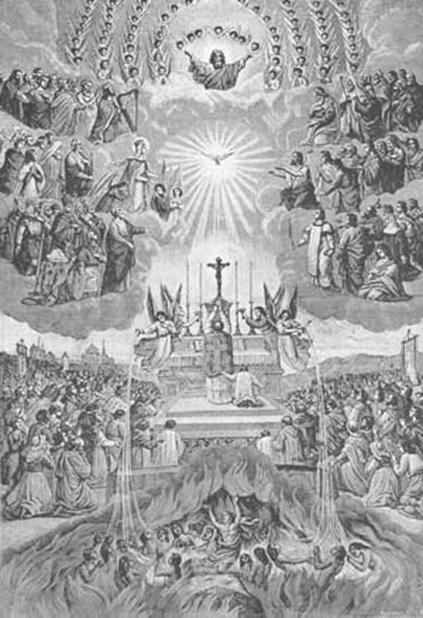
\includegraphics[scale=0.85]{gambar/purgatory2.jpg}
\end{center}

%\vspace{1cm}

\begin{center}
{\PTsmaller {Kasih, kerendahan hati, dan menurut pada kehendak Allah }}
\end{center}

\setlength{\parindent}{1cm}
\pagestyle{plain}
\begin{center}
%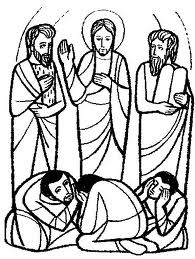
\includegraphics[scale=0.85]{gambar/TRANSFIGURASI.jpeg}
\end{center}
\chap{Bagaimana Injil Ditulis?}

\section*{Dokumen-dokumen}
Semua penerbitan Perjanjian Baru dan khususnya Injil, entah dalam bahasa Inggris, Spanyol, atau bahasa-bahasa lain, adalah hasil terjemahan dari teks-teks asli yang ditulis rlulam bahasa Yunani. Naskah-naskah kuno yang berisi teks-teks ini disalin berkali-kali, sampai akhirnya setiap teks dirapikan berkat penemuan mesin cetak; hal ini terjadi kira-kira tahun 456 di mana Guttenberg mencetak Kitab Suci yang pertama.

Orang-orang yang menyalin teks-teks ini tidak dapat menghindari beberapa kesalahan. Dengan membandingkan berbagai teks, pengelompokannya menurut perbedaan dan asal-usulnya, dan mengritiknya, kita dapat menentukan mana-mana saja teks asli yang diakui Gereja Katolik sebagai pernyataan iman para rasul dan sabda Allah. Pertanyannya: siapa yang menulis injil-injil yang pertama ini dan apa yang menjadi sumber mereka?

Beberapa naskah Perjanjian Baru yang hangus dari abad ke-4 telah diselamatkan. Naskah-naskah ini dikukuhkan oleh beberapa dokumen lainnya yang jauh lebih tua yang berisi paragraf-paragraf atau kadang-kadang kitab-kitab lengkap Perjanjian Baru. Selanjutnya, para penulis Kristen dari abad ke-2 dan ke-3 sering kali mengutip teks-teks suci yang sudah dikomentari. Injil Yohanes diperkiraan ditulis antara tahun 90 sampai 100, dan penggalan-penggalannya ditemukan di Mesir, sangat jauh dari tempat asalnya. Penggalan-penggalan itu tertanggal antara tahun 120-130.

Selanjutnya, kita akan memberi perhatian khusus pada Injil-injil, meskipun Injil-injil bukan merupakan tulisan Perjanjian Baru yang paling kuno saat ketiga Injil pertama ditulis pada tahun 50-70, Paulus sudah mengirim surat-surat aslinya.

\section*{Penulis-Penulis Injil}
Menarik untuk diperhatikan bahwa para ahli sejarah Gereja yang pertama sudah menyebutkan secara khusus orang-orang yang dianggap oleh tradisi sebagai penulis ketiga Injil sinoptik.

Pada tahun 110, Papias dari Herapolis (dekat Efesus) menulis: "Markus, penerjemah Petrus, menulis dengan tepat, meskipun tidak dalam susunan yang teratur, semua yang diingatnya mengenai perkataan-perkataan dan perbuatan-perbuatan Tuhan. Ia menemani Petrus yang mengajar sesuai dengan kebutuhan waktu, bukan dalam bentuk suatu komposisi, dan ia tidak melakukan kesalahan dalam memasukkan beberapa hal yang diingatnya. Matius mengumpulkan perkataan-perkataan Tuhan dalam bahasa Ibrani dan selanjutnya setiap orang menerjemahkannya sesuai dengan kemampuannya".

Pada tahun 185 Santo Ireneus, uskup dan martir, menulis, "Matius mewartakan injil di antara orang-orang Ibrani dan dalam bahasa mereka, sementara Petrus dan Paulus pergi keluar untuk menginjili Roma dan mendirikan gereja. Setelah mereka meninggalkan Roma, Markus, seorang murid dan penerjemah Petrus, menuliskan ajaran Petrus. Lukas, teman Paulus juga menulis sebuah kitab mengenai injil yang diajarkan oleh Paulus".

Sumber-sumber kuno yang mana kita masih bisa menambahnya, diteliti dengan seksama oleh banyak ahli kitab suci modern, dan akhirnya mereka diterima sekali lagi sebagai informasi benilai sejarah.

Selanjutnya, adalah suatu kesalahan untuk berpikir bahwa injil-injil telah ditulis dalam suatu kepingan oleh orang-orang seperti Matius, Markus atau Lukas yang pada suatu waktu tertentu memutuskan untuk mencatat dengan menuliskan pelayanan aktif dan ajaran Yesus.

\section*{Dari Tradisi Lisan ke Injil}
Kita tahu bahwa Yesus telah wafat dan Ia wafat tanpa menuliskan apapun. Yesus telah mengabdikan sebagian terbesar waktunya untuk membentuk kedua belas rasul yang telah dipilih-Nya. Mereka tinggal bersama Dia, sebagaimana kebiasaan dari murid-murid guru Yahudi. Yesus meminta mereka mempelajari ajaran-Nya dengan hati ketimbang melipat gandakan pengajaran-pengajaran-Nya, Yesus mengulangi kebenaran-kebenaran esensial dalam banyak cara. Kita tidak dapat meragukan itu bahwa setelah hari Pentakosta, perhatian mereka adalah memberi bentuk kepada perintah-perintah Yesus ini, yang kemudian menjadi katekismus Gereja Perdana. Pada awalnya para rasul memberi kesaksian tentang apa yang telah mereka lihat dan dengar. Lambat laun timbul kebutuhan untuk memiliki suatu catatan tertulis mengenai kesaksian mereka untuk menjaga ingatan: kita sendiri sering kali melakukan ini dalam suatu pertemuan, ketika sharing dari para peserta dicatat untuk kepentingan orang-orang yang tidak hadir.

Komunitas-komunitas Kristen, di Palestina berbicara dalam bahasa Aram atau Ibrani sesuai dengan daerah atau lingkungan. Dengan demikian tulisan yang pertama dimunculkan dalam kedua bahasa ini. Lambat laun teks-teks yang berkaitan dengan apa yang diucapkan dan diperbuat Yesus dikelompokkan kembali; dalam hal ini komunitas-komunitas Kristen pertama meneruskan dari kesaksian lisan menjadi teks tertulis: dan itu adalah injil.

Pada waktu itu komunitas-komunitas Kristen yang berbahasa Yunani telah menjadi kelompok mayoritas dan teks-teks kuno diterjemahkan ke daJam bahasa itu (Yunani).

\section*{Injii Yohanes}
Ketiga penulis injil yang pertama tidak hanya berbeda dalam fokus mereka tetapi juga agak berbeda dalam menyajikan perbuatan-perbuatan dan perkataan-perkataan Yesus; sebetulnya masing-masing mempunyai teologi-nya sendiri, caranya mengenal Yesus, dari pandarig an 'yang mendalam' serta kesaksian pribadi inilah yang akhirnya menentukan perbedaan.

Dalam Injil Yohanes kita menemukan, bagian-bagian suaru injil kuno yang sesederhana lnjil Markus, dengan lebih banyak perbuatan daripada perkataan Yesus, yang mungkin telah disampaikan kepada komunitas umat Kristen di Samaria, dan yang ditulis dalam bahasa Aram. Inilah dasar dimanu Yohanes mengembangkan uraian yang panjang mengenai Yesus yang memperlihatkan bahwa keselamatan mengubah umat manusia dan memperbarui ciptaan.

\section*{Apakah kita dapat mempercayai perkataan Injil?}
Sebagian besar dari kita mungkin sudah menanyakan ini: mengapa kita mempunyai empat kesaksian ketimbang satu, dan apa nilainya masing-masing, Mengikuti apa yang baru saja kita katakan akan lebih mudah mengerti apa yang menyusul:
\begin{itemize}
\item Tidak semua perbuatan dan perkataan Yesus ditemukan dalam injil.
\item Berkenaan dengan kata-Kata Yesus, setiap penulis injil mengungkapkannya dalam caranya sendiri dan menerapkannya untuk pemahaman yang lebih baik bagi para pembacanya.
\item Kejadian-kejadian tidak selalu diceritakan berurutan sesuai dengan terjadinya; dan hal-hal yang dikatakan Yesus pada kesempatan yang berbeda dapat digabungkan dalam nas yang sama.
\end{itemize}

Ini tidak mengatakan bahwa kita tidak dapat mempercayai kesaksian para penulis injil. Kita tidak diberi sebuah "foto", sebuah rekaman kata-kata Yesus, tetapi sebaliknya empat pandangan yang berbeda yang saling melengkapi. Mengapa khawatir jika terdapat pertentangan-pertentangan tertentu dalam perincian-perincian, Jika di pintu gerbang Yeriko terdapat satu atau dua orang buta, apa bedanya dalam pesan pokok yang disampaikan?.

\section*{Tempat Khusus Injil-injil dalam Literatur}
Injil-injil adalah karya kekecualian khusus diantara karya-karya tulisan sepanjang zaman. Perbandingan-perbandingan tulisan-tulisan lain dari zamannya, Kristen atau bukan, memperlihatkan suatu kontras luar biasa -- dalam injil, kesederhanaan keinginan untuk bersabar, sementara teks-teks yang lain, lebih mengutamakan apa-apa yang hebat, kompleks dan tidak berakar rumput. Seorang filsuf modern -- bukan orang beriman -- bertanya mengapa tidak dapat lebih banyak mukjizat di dalam Injil. Injil-injil memiliki jaminan keasliannya sendiri. Mempertimbangkan apa yang dikatakan dalam paragraf terdahulu, kritik modern belum dapat menemukan kekeliruan di dalam Injil meskipun ia telah memeriksanya dengan teliti dengan menggunakan kaca pembesar selama lebih dari satu abad. Apalagi: injil menyapa kita dengan suatu perasaan penuh arti setiap kali kita mampu membuka diri kita kepadanya.

\section*{Mereka Meragukannya}
Masih banyak orang yang mempertanyakan kesaksian Injil. Kadang-kadang disebabkan karena mereka mengira mereka melihat pertentangan-pertentangan di dalam Injil; tetapi lebih sering karena tampaknya tidak mungkin bagi mereka untuk menerima mukjizat-mukjizat. Bahkan di antara orang-orang beriman yang mempelajari Injil, beberapa orang memiliki sejumlah keraguan berkaitan dengan nilai historis segala sesuatu yang dapat disebut mukjizat dalam arti harfiah.

Hal ini mungkin disebabkan oleh kenyataan bahwa mereka telah dididik dalam budaya "ilmiah" yang hanya mengandalkan pengertian manusia untuk mengatasi setip masalah. dalam suatu dunia yang melindungi dirinya dengan asuransi, sedikit yang diharapkan dari Allah dan Allah tidak melipatgandakan mukjizat.

Mereka berpikir sebagai berikut: Jika sekarang saya tidak dapat melihat apa pun yang sama dengan apa yang terjadi dalam Injil, bagaimana saya bisa percaya bahwa hal-hal semacam itu juga terjadi kemudian? Segala sesuatu barangkali berbeda jika mereka melibatkan diri di dalam komunitas-komunitas Kristen yang miskin atau tertindas. DI sana mereka mungkin dapat menyaksikan campur tangan Allah yang terus-menerus demi kebaikan orang-orang yang hanya dapat berharap kepada-Nya saja. Sesungguhnya, dalam kumuniras-komuniras ini dikatakan: Jika hari itu Allah mengerjakan mukjizat-mukjizat Itu, mengapa Ia tidak mungkin mengerjakannya pada zaman Yesus seturut kehendak-Nya?

Sesungguhnya, tidak mungkin mempelajari Injil secara parsial, sebagaimana yang bisa lakukan terhadap buku-buku lainnya karena lnjil mengajukan pertanyaan mengenai keseluruhan hidup kita dan bukann hnaya mengenai gagasan-gagasan tertentu. Jika kita mengambil bagian dalam iman pararasul, kita seharusnya tidak mengalami kesulitan untuk menerima Kitab Suci seraya menyadari pertanyaan-pertanyaan yang kritis. Tetapi, jika kita tidak memenuhi persyaratan-persyaratan yang akan memungkinkan kita untuk melihat Allah, kita merasa risih sampai menemukan alasan-alasan untuk mengurangi kesaksian Injil kepada sesuatu yang tampak masuk akal; yang berarti bahwa aJasan tersebut tidak akan mempertanyakan pendirian kita dalam hidup. Itulah sebabnya banyak orang, meskipun mereka mengagumi Injil dan menolak untuk menganggapnya sebagai suatu kebohongan, mencari ribuan aJasan unruk menyangkal apa yang tampaknya mengguncangkan mereka; kesaksian lnjil tentang Allah menjadi manusia; seorang Allah yang bergaul di antara manusia dan yang membangkitkan orang dari mati.

\section*{Beberapa Penolakan}
Oleh karena itu, mereka secara khusus berpegang teguh pada dua argumen pokok:
\begin{enumerate}
\item Mereka mengatakan bahwa Injil ditulis bertahun-tahun setelah kematian Yesus di mana telah terbentuk sebuah gambaran yang suci tentang Yesus. Dengan demikian, mereka tidak menyatakan realitas Yesus yang sesungguhnya kepada kita, melainkan iman Gereja ~ada abad pertama. (Bandingkan dengan apa yang telah kita katakan mengenai waktu penulisan Injil.
\item Mereka juga mengatakan bahwa Injil adalah tulisan-tulisan yang dimaksudkan sebagai katekismus dan pengajaran untuk orang-orang Kristen: fakta-fakta yang bertujuan untuk mendukung apa yang mereka ajarkan. Karena itu, tidaklah penting apakah Yesus berjalan di atas air atau tidak; episode Itu ditulis untuk menunjukkan bahwa Yesus memiliki kekuasaan Ilahi.
\end{enumerate}

\section*{Tetapi, bagaimana dengan para rasul?}
Mereka telah menjadi saksi-saksi Yesus,dan peranan mereka adalah untuk tetap menjadi saksi-saksi resmi-Nya di dalam Gereja. Mereka tahu persis apa sesungguhnya yang telah terjadi; apakah mereka harus tetap diam semen tara orang-orang membelokkan sejarah Yesus? Jaminan Injil ditemukan dalam struktur hakiki Gereja Katolik, yang tidak pemah merupakan suatu kelompok umat beriman yang secara spontan dikendalikan oleh antusiasme atau oportunisme.

Injil berasal dari tradisi para rasul dan Gereja tetap memelihara tradisi karena Gereja mengakuinya di dalam Injil. Dalam tahun-tahun itu dan dalam abad benkutnya, Injil-injil yang lain ditulis: Injil Petrus, Injil Thomas, Injil Nikodemus, Injll Pertama Yakobus. Akan tetapi, Gereja tidak menerima Injil-injil ini karena peristiwa-peristiwa fantastis yang tertulis di dalamnya, atau karena orientasi teologis yang tidak sesuai dengan ajaran yang diterima dari para rasul. 
\chap{Bagaimana menginterpretasikan Kitab Suci menurut pengajaran Gereja Katolik?}
\section{Perkenalan dengan Kitab Suci}
Orang mengatakan bahwa tak kenal maka tak sayang. Maka agar kita dapat mengasihi Tuhan, kita perlu mengenal Dia. Sekarang pertanyaannya, bagaimana caranya kita mengenal Allah?  Agaknya Tuhan memahami bahwa manusia akan mempunyai pertanyaan semacam ini dalam hatinya, sehingga Allah-lah yang pertama- tama melakukan inisiatif: Ia mewahyukan Diri-Nya, melalui alam semesta, melalui suara hati nurani dan yang secara khusus, melalui Wahyu umum yang diberikan kepada Gereja.
\subsection{Apakah Kitab Suci itu?}
Kita sering mendengar bahwa Kitab Suci adalah "Wahyu Allah". Wahyu atau pernyataan Allah tentang diri-Nya ini tidak terlepas dari kenyataan bahwa manusia diciptakan menurut gambar dan rupa Allah (Kej 1: 26). Artinya kita adalah mahluk rohani yang diciptakan menurut gambaran Allah, yang dilengkapi oleh akal budi dan kehendak bebas, sehingga kita dapat mengetahui, memilih dan mengasihi. Dengan demikian, kita manusia dapat menyimpulkan bahwa Tuhan Sang Pencipta itu ada, dengan melihat segala ciptaan-Nya yang ada di sekitar kita. Keberadaan Tuhan juga diketahui dengan memperhatikan suara hati nurani dalam setiap orang, di mana Tuhan menuliskan hukum-hukum-Nya untuk menyatakan hal yang benar dan yang salah; inilah wahyu yang universal. Selanjutnya, Tuhan juga secara khusus memberikan wahyu yang merupakan pernyataan akan diri-Nya dan kehendak-Nya bagi manusia untuk mencapai tujuan akhir yang direncanakan-Nya. Wahyu ini disampaikan kepada manusia sejak awal sejarah manusia sampai sekarang; yaitu  melalui para nabi, yang mencapai puncaknya di dalam Yesus Kristus Putera-Nya, dan wahyu ini yang kemudian dilanjutkan oleh para rasul Kristus.

Wahyu umum ini adalah wahyu Allah yang khusus diberikan kepada umat manusia agar manusia dapat mengenal siapa diri-Nya dan rencana-Nya untuk menyelamatkan manusia. Wahyu umum ini bermula dari wahyu yang diberikan kepada para nabi, dan berakhir dengan wafatnya rasul Kristus yang terakhir. Wahyu umum ini terdiri dari dua jenis, yang tergantung dari cara penyampaiannya; yaitu Kitab Suci (tertulis) dan Tradisi Suci (lisan). Maka kita ketahui ketiga hal ini:
\begin{enumerate}
\item Kitab Suci adalah Wahyu ilahi yang disampaikan secara tertulis di bawah inspirasi Roh Kudus.
\item Tradisi Suci adalah Wahyu ilahi yang tidak tertulis, namun yang diturunkan oleh para rasul sejak awal oleh inspirasi Roh Kudus, sesuai dengan yang mereka terima dari Yesus dan yang kemudian diturunkan kepada para penerus mereka.
\item Maka kita ketahui sekarang bahwa untuk menerima wahyu Allah secara lengkap, kita tidak hanya perlu Kitab Suci, namun juga Tradisi Suci, dan pihak wewenang mengajar Gereja (Magisterium) yang dapat secara benar mengartikan wahyu ilahi tersebut. Ketiga hal ini disebut sebagai pilar iman, yang ditujukan untuk menjaga dan mengartikan wahyu publik dari Allah ini di dalam kemurniannya.
\end{enumerate}

\subsection{Kitab Suci yang adalah Sabda Allah itu terdiri atas Perjanjian Lama dan Perjanjian Baru}
Pernahkah anda membaca novel, namun hanya membaca bagian akhirnya saja? Walaupun mungkin anda dapat menangkap bagian yang terpenting dari kisah tersebut, namun tentu, kisah tersebut akan lebih dapat dipahami, jika anda membaca buku tersebut mulai dari bagian awal. Demikianlah halnya dengan Kitab Suci yang merupakan Sabda Allah yang tertulis tentang rencana keselamatan Allah yang dimulai sejak awal mula penciptaan dunia, sampai penggenapannya di dalam diri Kristus.

Oleh karena itu, untuk mempelajari Kitab Suci, kita perlu melihat kaitan antara Perjanjian Lama (sebelum kedatangan Kristus) dan Perjanjian Baru (saat dan setelah kedatangan Kristus), dan antara ayat yang satu dengan ayat yang lainnya, untuk mendapat pengertian yang menyeluruh dan pemahaman yang benar akan Sabda Allah itu. Perjanjian Lama (PL) yang melatar-belakangi Perjanjian Baru (PB), merupakan satu kesatuan dengan Perjanjian Baru. Sebab "Perjanjian Baru terselubung dalam Perjanjian Lama, sedangkan Perjanjian Lama tersingkap dalam Perjanjian Baru.". Sama seperti suatu kisah tidak akan lengkap jika hanya dibaca awalnya saja, atau akhirnya saja, tanpa memperhatikan kaitannya, demikian juga Kitab Suci hanya akan dapat kita pahami secara menyeluruh dalam kesatuan antara PL dan PB, dan dalam kaitan satu ayat dengan ayat yang lain.

\subsection{Penulisan Kitab Suci melibatkan akal budi para penulisnya}
Kitab Suci merupakan Sabda Allah yang disampaikan melalui tulisan penulis kitab yang ditunjuk oleh Allah untuk menuliskan hanya yang diinginkan oleh Tuhan. Namun demikian, ini melibatkan juga kemampuan sang penulis tersebut dalam hal gaya bahasa, cara penyusunan, latar belakang budayanya, dst. Maka jika kita ingin memahami Kitab Suci, kita perlu mengetahui makna yang disampaikan oleh para pengarang kitab dan apakah yang ingin disampaikan oleh Allah melalui tulisannya. Karena Kitab Suci bersumber pada Allah yang satu, maka kita harus melihat keseluruhan Kitab Suci, walaupun ditulis oleh orang yang berbeda- beda, sebagai satu kesatuan yang saling melengkapi. Inilah yang menjadi dasar bagaimana kita memperoleh pengertian yang mendalam tentang Kitab Suci, dan dengan cara demikianlah jemaat awal mengartikan Kitab Suci.

\subsection{Kitab Suci itu diberikan kepada Gereja sebagai pedoman}
Rasul Paulus memberikan alasan kepada kita untuk mempelajari Kitab Suci yaitu, "Segala tulisan yang diilhamkan Allah memang bermanfaat untuk mengajar, untuk menyatakan kesalahan, untuk memperbaiki kelakuan dan untuk mendidik orang dalam kebenaran" (2 Tim 3:16) agar kita yang menjadi umat-Nya diperlengkapi untuk setiap perbuatan baik. Dengan demikian, Kitab Suci mendapatkan tempat yang begitu tinggi di dalam Gereja Katolik, yang dapat kita lihat dari dokumen-dokumen Gereja yang senantiasa mempunyai sumber dari Kitab Suci disamping Tradisi Suci, dan kita dapat melihat secara jelas dalam liturgi Gereja. Paus Benediktus XVI dalam pengajaran apostoliknya, Verbum Domini, mengajarkan bahwa Kitab Suci mendapatkan tempat di dalam sakramen-sakramen, liturgi, brevier, buku-buku doa dan pemberkatan, lagu-lagu, dll.

\section{Prinsip umum yang harus dipegang}
\subsection{Gereja ada terlebih dahulu sebelum Kitab Suci.}
Jika kita mempelajari sejarah Gereja, kita akan mengetahui bahwa Tradisi Suci, yaitu pengajaran iman Kristiani yang berasal dari pengajaran lisan Kristus dan para rasul itu sudah ada terlebih dahulu daripada pengajaran yang tertulis. Demikian pula, Gereja sudah ada terlebih dahulu sebelum keberadaan kitab-kitab Perjanjian Baru. Yesus tidak membentuk Kitab Suci, namun Yesus membentuk Gereja, yang Ia dirikan di atas Rasul Petrus (lih. Mat 16:18). Gereja pulalah yang menentukan kanon seluruh Kitab Suci, baik Perjanjian Lama maupun Perjanjian Baru. Para pengarang/ penulis suci dari kitab-kitab Perjanjian Baru adalah para anggota Gereja yang diilhami oleh Tuhan, sama seperti para penulis suci yang menuliskan kitab-kitab Perjanjian Lama.

\subsection{Kitab Suci memberitahukan kepada kita pentingnya Tradisi Suci, yaitu pengajaran lisan para rasul, sebab tidak semua ajaran Kristus terekam dalam Kitab Suci.}
Jemaat mula-mula "bertekun dalam pengajaran rasul-rasul… " (Kis 2:42, lih. 2 Tim 1:14), dan ini sudah terjadi sebelum kitab Perjanjian Baru ditulis, berabad – abad sebelum kanon Perjanjian Baru ditetapkan di akhir abad ke 4. Kitab Suci juga mengatakan bahwa pengajaran para rasul disampaikan secara lisan, "Apa yang telah engkau dengar dari padaku di depan banyak saksi, percayakanlah itu kepada orang-orang yang dapat dipercayai, yang juga cakap mengajar orang lain." (2 Tim 2:2); dan bahwa pengajaran para rasul tersebut disampaikan "baik secara lisan, maupun secara tertulis." (2 Tes 2:15; lihat juga bahwa ‘ajaran yang diteruskan/ diberitakan melalui pembicaraan’ oleh para rasul inilah Tradisi suci -1 Kor 11:2, 23; 2 Yoh 12, 3 Yoh 13)

"Masih banyak hal-hal lain lagi yang diperbuat oleh Yesus, tetapi jikalau semuanya itu harus dituliskan satu per satu, maka agaknya dunia ini tidak dapat memuat semua kitab yang harus ditulis itu." (Yoh 21:25). Kitab Perjanjian Baru sendiri mengacu kepada Tradisi suci, yaitu pada saat mengutip perkataan Yesus yang tidak terekam pada Injil, yaitu pada Kis 20:35, di mana rasul Paulus meneruskan perkataan Yesus "Adalah lebih berbahagia memberi daripada menerima"; yaitu perkataan Yesus yang tidak tertulis dalam Injil.

\subsection{Kitab Suci sendiri mengatakan bahwa Kitab Suci memerlukan pihak yang mempunyai otoritas untuk menginterpretasikannya}
Rasul Petrus mengatakan bahwa ada hal-hal di dalam Kitab Suci yang memang sulit untuk dicerna (lih. Kis 8:30-31; 2 Pet 1:20-21; 2 Pet 3:15-16), dan ketidakhati-hatian dalam penafsiran akan mendatangkan kesalahan yang fatal. Berapa banyak kita mendengar dari agama lain, yang menggunakan Kitab Suci untuk menyanggah kebenaran iman Kristen, seperti tentang ajaran Tritunggal Maha Kudus, ataupun bahwa Yesus adalah sungguh- sungguh Tuhan.

\subsection{Kristus memberikan otoritas kepada Gereja yang dimulai dari para rasul-Nya untuk mengajar dalam nama-Nya.}
Gereja akan bertahan sampai pada akhir jaman, dan Kristus oleh kuasa Roh Kudus akan menjaganya dari kesesatan (lih. Mat 16:18; 18:18; 28:19-20; Luk 10:16; Yoh 14:16). Karena itu, Kristus memberikan kuasa wewenang mengajar kepada Magisterium Gereja yang terdiri dari para rasul dan para penerusnya. Magisterium/ Wewenang mengajar ini hanya ada untuk melayani Sabda Allah, sehingga ia tidak berada di atas Kitab Suci maupun Tradisi Suci, namun melayani keduanya. Prinsip fungsi Magisterium ini hanya seperti wasit dalam pertandingan sepak bola: ia tidak mengatasi peraturan, namun hanya menjaga agar peraturan dijalankan semestinya.

Hal yang sama ditegaskan oleh Paus Benediktus XVI dalam pengajaran Apostoliknya, Verbum Domini. Paus menegaskan bahwa apa yang tertulis di dalam Kitab Suci bukanlah sesuatu yang dapat diinterpretasikan oleh masing-masing individu dengan bebas tanpa melihat apa yang menjadi pandangan Gereja. Karena Sabda Allah yang bersumber pada Roh Kudus diberikan kepada Gereja. Oleh Roh Kudus menjadi jiwa dari Gereja, Gereja menentukan buku-buku yang masuk ke dalam kanon Kitab Suci. Dengan demikian, Gereja mempunyai otoritas untuk menginterpretasikan Kitab Suci sesuai dengan maksud yang ingin disampaikan oleh Roh Kudus. Hal yang sama juga ditegaskan oleh St. Agustinus yang mengatakan "\textit{I would not believe the Gospel, had not the authority of the Catholic Church led me to do so}"

Jika kita melihat sejarah, maka kita dapat melihat bahwa Kitab Suci yang ada pada kita sekarang terbentuk pertama kali menurut kanon yang ditetapkan oleh Paus Damasus pada tahun 382, Konsili Hippo (393), Carthago (397) dan Kalsedon/ Chalcedon (451) yang kemudian diteguhkan oleh banyak konsili sampai Konsili Trente (1545- 1563). Maka Gerejalah, atas ilham Roh Kudus, yang menentukan kitab- kitab mana saja yang diinspirasikan oleh Roh Kudus, sehingga dapat termasuk dalam Kitab Suci. Sebelum Kitab Suci ditulis, Gereja mengandalkan Tradisi Suci, yaitu pengajaran lisan para rasul. Ini adalah bukti penerapan ayat 1 Tim 3:15, yaitu bahwa Gereja-lah (bukan Kitab Suci) yang menjadi tiang penopang dan tonggak kebenaran. Jadi mengatakan bahwa Kitab Suci saja "cukup" atau "hanya satu-satunya" sebagai pedoman iman, itu tidaklah benar, sebab asal mula Kitab Suci itu sendiri melibatkan Tradisi Suci dan Gereja, yang dipimpin oleh Magisterium.

\subsection{Kitab Suci mengacu kepada Tradisi Suci untuk menyelesaikan masalah di dalam jemaat}
Saat terjadinya krisis dalam jemaat di sekitar tahun 40-an, kitab Perjanjian Baru belum ada, dan Kristus sendiri tidak pernah mengajarkan secara eksplisit tentang sunat. Namun atas inspirasi Roh Kudus, atas kesaksian Rasul Petrus, maka Konsili Yerusalem menetapkan bahwa sunat tidak lagi diperlukan bagi para pengikut Kristus (Kis 15). Konsili inilah yang menginterpretasikan kembali Kitab Suci Perjanjian Lama yang mengharuskan sunat (lih. Kej 17, Kel 12:48) dengan terang Roh Kudus dan penggenapannya oleh Kristus dalam Perjanjian Baru, sehingga ketentuan sunat tidak lagi diberlakukan. Di dalam Konsili itu, Magisterium Gereja: para rasul dan penerusnya, dan pemimpin Gereja lainnya berkumpul untuk memeriksa Sabda Tuhan, yang tertulis atau yang tidak, dan membuat suatu pengajaran apostolik sesuai dengan ajaran Kristus.

\subsection{Maka di sini terlihat bahwa Gereja/ jemaat (bukan Kitab Suci saja) adalah "tiang penopang dan dasar kebenaran." (1 Tim 3:15)}
Kristus mendirikan Gereja, dan bukannya menulis Kitab Suci, tentu juga ada maksudnya, bahwa Gereja-lah yang dipercaya oleh Kristus untuk mengajar dan menafsirkan semua firman-Nya.

\subsection{Kitab Suci tidak mengatakan bahwa Kitab Suci adalah satu-satunya sumber Sabda/ Firman Tuhan.}
Kristus itu sendiri adalah Firman Allah (lih. Yoh 1:1, 14) dan dalam 1 Tes 2:13 Rasul Paulus mengatakan bahwa ia telah menyampaikan pemberitaan Firman Allah ("when you received the Word of God which you heard from us"- RSV) dan pemberitaan Firman Allah (melalui pendengaran) yang disampaikan oleh para rasul adalah Tradisi Suci.

\section{Prinsip untuk menginterpretasikan Kitab Suci}
\subsection{Cara umum:}
Konsili Vatikan II mengajarkan tiga cara umum untuk menafsirkan Kitab Suci sesuai dengan Roh Kudus yang mengilhaminya:
\begin{enumerate}
\item Memperhatikan isi dan kesatuan seluruh Kitab Suci

Kita harus mengartikan ayat tertentu dalam Kitab Suci dalam kaitannya dengan pesan Kitab Suci secara keseluruhan. Mengartikan satu paragraf atau bahkan satu kalimat saja namun tidak memperhatikan kaitannya dengan ayat yang lain, dapat berakibat fatal. Contohnya, seorang atheis mengutip Mzm 14:1, dan berkata "Tidak ada Allah". Tetapi sebenarnya, keseluruhan kalimat itu berkata, "Orang bebal berkata dalam hatinya: "Tidak ada Allah". Maka arti yang disampaikan dalam Kitab Suci tentu sangat berbeda dengan pengertian orang atheis tersebut.

\item Membaca Kitab Suci dalam terang Tradisi hidup seluruh Gereja

Banyak ahli Kitab Suci di jaman modern yang tidak mengindahkan interpretasi yang berakar dari tradisi Gereja. Mereka berpikir seolah-olah baru pada saat mereka menginterpretasikan Kitab Suci, Roh Kudus memberikan pengertian yang paling "asli", sedang interpretasi pada abad- abad yang lalu itu keliru. Sikap ini tentunya tidak mencerminkan kerendahan hati. Gereja mengajarkan bahwa kita harus menginterpretasikan Kitab Suci sesuai dengan Tradisi hidup seluruh Gereja, sebab "Kitab suci lebih dulu ditulis di dalam hati Gereja daripada di atas pergamen (kertas dari kulit)". Di dalam Tradisi Suci inilah Roh Kudus menyatakan kenangan yang hidup tentang Sabda Allah dan interpretasi spiritual dari Kitab Suci. Tradisi Suci tercermin dari tulisan Para Bapa Gereja, dan ajaran- ajaran definitif yang ditetapkan oleh Magisterium, seperti yang dihasilkan dalam Konsili-konsili, Bapa Paus maupun yang dijabarkan dalam doktrin Gereja.

\item Memperhatikan "analogi iman"

Analogi iman maksudnya adalah bahwa wahyu Allah berisi kebenaran- kebenaran yang konsisten dan tidak bertentangan satu sama lain. Gereja Katolik percaya bahwa Roh Kudus yang meng-inspirasikan Kitab Suci adalah Roh Kudus yang sama, yang membimbing dan menjaga wewenang mengajar Gereja (Magisterium), yang juga bekerja dalam Tradisi Suci Gereja. Maka tidak mungkin ajaran Gereja Katolik bertentangan dengan Kitab Suci, karena Roh Kudus tidak mungkin bertentangan dengan diri-Nya sendiri. Juga, karena Gereja menjaga kemurnian ajaran dalam Kitab Suci, maka untuk meng-interpretasikan Kitab Suci, kita harus melihat kaitannya dengan ajaran/ doktrin Gereja.

Analogi iman yang berdasarkan ajaran Gereja berperan sebagai "penjaga" yang membantu kita agar kita tidak sampai salah jalan dalam meng-interpretasikan Kitab Suci. Ibaratnya, seperti pagar yang membatasi rumah kita dengan dunia luar yang penuh dengan anjing galak. Di dalam halaman rumah, kita tetap dapat beraktivitas, anak-anak dapat bermain dengan bebas, namun aman dari bahaya. Maka dengan berpegang pada ajaran Gereja, kita tetap mempunyai kebebasan dalam menginterpretasikan ayat-ayat Kitab Suci, namun kita dapat yakin bahwa interpretasi kita tidak salah, ataupun tidak bertentangan dengan kebenaran yang diwahyukan. Keyakinan ini merupakan karunia yang diberikan kepada kita, jika kita setia berpegang pada pengajaran Gereja yang disampaikan oleh Magisterium (Wewenang mengajar Gereja). Magisterium inilah yang bertugas menginterpretasikan Sabda Allah dengan otentik, baik yang tertulis (Kitab Suci) maupun yang lisan (Tradisi Suci), dengan wewenang yang dilakukan dalam nama Tuhan Yesus agar Sabda itu dapat diteruskan sesuai dengan yang diterima oleh para rasul.
\end{enumerate}

\subsection{Menghindari dualisme hermenetik sekular/ ‘secularized hermeneutic’ dan interpretasi fundamentalis/"fundamentalist interpretation"}
Paus Benediktus XVI dalam ekshortasi apostoliknya, Verbum Domini menekankan dua kesalahan ekstrem yang tidak boleh dilakukan oleh umat Katolik dalam menginterpretasikan Kitab Suci. Dua kesalahan ini adalah hanya berdasarkan metoda sekular dan metoda fundamentalisme.
\begin{enumerate}
\item Metoda historical-criticism yang terpisah dari teologi

Metode sekular yang terpisah dari teologi ini menekankan sisi sejarah dari Kitab Suci, sehingga Kitab Suci hanya dilihat sebagai buku dari masa lampau yang tidak mempunyai kaitan dengan saat ini. Pendekatan yang ilmiah dengan mengesampingkan sisi-sisi Ilahi dari Kitab Suci membuat metode ini kehilangan apa yang menjadi dasar untuk mengerti Kitab Suci – yaitu iman – yang pada akhirnya menolak campur tangan Tuhan dalam sejarah manusia. Inilah sebabnya, Paus Yohanes Paulus II – dalam ensiklik Fides et Ratio – dan Paus Benediktus XVI menekankan harmoni antara iman dan akal budi. Menyandarkan metoda ilmiah dalam menginterpretasikan Kitab Suci tanpa dibarengi iman, mereduksi sisi Ilahi dari Kitab Suci menjadi buku sejarah atau hanya menjadi buku literatur biasa. Sebagai contoh: Ketika di Kitab Suci dikatakan bahwa Yesus memberi makan lima ribu orang (Mt 14:15-21; Mk 6:34-44), maka metoda ini cenderung untuk mereduksi sisi Ilahi dari Kristus dan kemudian menjelaskannya dengan sesuatu yang lebih ilmiah, seperti orang-orang yang ada berkumpul mengeluarkan bekal masing-masing dan kemudian saling berbagi.

\item Metode fundamentalisme

Metode fundamentalisme mengambil kata demi kata di Kitab Suci dan menganggap kata demi kata dalam Kitab Suci adalah didikte oleh Tuhan tanpa melihat bahwa penulisan Kitab Suci senantiasa di dalam konteks sejarah pada waktu tulisan tersebut dibuat. Penolakan akan sisi sejarah dan juga penolakan akan Gereja sebagai pemberi interpretasi Kitab Suci yang otentik membuat metode ini menjadi sangat subyektif yang mengarah bahwa interpretasi pribadinya sendiri adalah yang paling benar. Metoda ini juga dapat menyebabkan kegagalan untuk melihat Sabda Allah dalam konteks keseluruhan. Sebagai contoh, ketika Yesus mengatakan "Tetapi tentang hari dan saat itu tidak seorangpun yang tahu, malaikat-malaikat di sorga tidak, dan Anakpun tidak, hanya Bapa sendiri." (Mt 24:36), maka metoda ini mempunyai tendensi untuk mengatakan bahwa Yesus memang tidak mengetahui kapan akhir dunia terjadi, tanpa melihat kompleksitas dari kodrat Yesus yang sungguh Allah dan sungguh manusia. Karena mereka juga tidak mau melihat komentar Kitab Suci dari Bapa Gereja dan Magisterium Gereja, maka mereka akan mengeraskan hati bahwa interpretasi merekalah yang paling benar.
\end{enumerate}

\subsection{Ke-4 Prinsip menginterpretasikan Kitab Suci}
Secara umum, Kitab Suci mempunyai dua macam arti. Yang pertama disebut ‘literal/ harafiah’ sedangkan yang kedua disebut sebagai ‘spiritual/ rohaniah’. Kemudian arti rohaniah ini terbagi menjadi 3 macam, yaitu: alegoris, moral dan anagogis. Ke-empat macam arti ini secara jelas menghubungkan Perjanjian Lama dan Perjanjian Baru.


a. Arti literal/ harafiah.
Arti harafiah adalah arti yang berdasarkan atas penuturan teks yang ada secara tepat. Mengikuti ajaran St. Thomas Aquinas, kita harus berpegang bahwa, "Tiap arti [Kitab Suci] berakar di dalam arti harafiah."[16] Jadi dalam membaca Kitab suci, kita harus mengerti akan arti kata-kata yang dimaksud secara harafiah yang ingin disampaikan oleh pengarangnya, baru kemudian kita melihat apakah ada maksud rohani yang lain. Arti rohani ini timbul berdasarkan arti harafiah.
b. Arti alegoris
Arti alegoris adalah arti yang lebih mendalam yang diperoleh dari suatu kejadian, jika kita menghubungkan peristiwa tersebut dengan Kristus. Contohnya:
1.    Penyeberangan bangsa Israel melintasi Laut Merah adalah tanda kemenangan yang diperoleh umat beriman melalui Pembaptisan (lih.Kel14:13-31; 1Kor 10:2).
2.    Kurban anak domba Paska di Perjanjian Lama merupakan gambaran kurban Yesus Sang Anak Domba Allah pada Perjanjian Baru (Kel 12: 21-28; 1 Kor 5:7).
3.    Abraham yang rela mengurbankan anaknya Ishak adalah gambaran dari Allah Bapa yang rela mengurbankan Yesus Kristus Putera-Nya (Kej 22: 16; Rom 8:32).
4.    Tabut Perjanjian Lama adalah gambaran dari Bunda Maria, Sang Tabut Perjanjian Baru. Karena pada tabut Perjanjian Lama tersimpan dua loh batu kesepuluh perintah Allah (Kel 25:16), roti manna (Kel 25:30), tongkat Harun sang imam(Ibr 9:4); sedangkan pada rahim Maria Sang Tabut Perjanjian Baru tersimpan Sang Sabda yang menjadi manusia (Yoh 1:14), Sang Roti Hidup (Yoh 6:35), Sang Imam Agung (Ibr 8:1).
c. Arti moral
Arti moral adalah arti yang mengacu kepada hal-hal yang baik yang ingin disampaikan melalui kejadian- kejadian di dalam KItab Suci. Hal-hal itu ditulis sebagai "contoh bagi kita \dots sebagai peringatan" (1 Kor 10:11).
1.    Ajaran Yesus agar kita duduk di tempat yang paling rendah jika diundang ke pesta (Luk 14:10), maksudnya adalah agar kita berusaha menjadi rendah hati.
2.    Peringatan Yesus yang mengatakan bahwa ukuran yang kita pakai akan diukurkan kepada kita (Mrk 4: 24) maksudnya agar kita tidak lekas menghakimi orang lain.
3.    Melalui mukjizat Yesus menyembuhkan dua orang buta, yang berteriak-teriak, "Yesus, Anak Daud, kasihanilah kami!" (Mat 20: 29-34) Yesus mengajarkan agar kita tidak lekas menyerah dalam doa permohonan kita.
d. Arti anagogis
Arti anagogis adalah arti yang menunjuk kepada surga sebagai ‘tanah air abadi’. Contohnya adalah:
1.    Gereja di dunia ini melambangkan Yerusalem surgawi (lih. Why 21:1-22:5).
2.    Surga adalah tempat di mana Allah akan menghapuskan setiap titik air mata (Why 7:17).
e. Hubungan antara ke-empat arti Kitab Suci
Berikut ini adalah pepatah yang berasal dari Abad Pertengahan tentang arti ke-empat arti Kitab Suci. "Huruf [dari kata letter/ literal] mengajarkan kejadian; apa yang harus kau percaya, alegori; moral, apa yang harus kau lakukan; ke mana kau harus berjalan, anagogi."[17]
4. Contoh interpretasi Kitab Suci dengan menggunakan ke-4 prinsip
Maka semua kejadian di dalam Kitab Suci memiliki makna harafiah, walaupun dapat mengandung arti rohaniah juga. Contohnya adalah kisah Allah menurunkan roti manna di padang gurun (Kel 16).[18]
1.    Secara harafiah, memang Allah memberi makan bangsa Israel dengan manna yang turun dari langit selama 40 tahun saat mereka mengembara di padang gurun.
2.    Secara alegoris, roti manna menjadi gambaran Ekaristi, di mana Yesus sebagai Roti Hidup adalah Roti yang turun dari surga (Yoh 6:51), menjadi santapan rohani kita umat beriman yang masih berziarah di dunia ini.
3.    Secara moral, kisah ini mengajarkan kita untuk tidak cepat mengeluh dan bersungut-sungut (Kel 16:2-3) kepada Allah. Umat Israel yang bersungut-sungut akhirnya dihukum Allah sehingga tak ada dari generasi mereka yang dapat masuk ke tanah terjanji (selain Yoshua dan Kaleb).
4.    Secara anagogis, kita diingatkan bahwa seperti roti manna yang berhenti diturunkan setelah bangsa Israel masuk ke Tanah Kanaan, maka Ekaristipun akan berakhir pada saat kita masuk Surga, yaitu saat kita melihat Tuhan dalam keadaan yang sebenarnya (1 Yoh 3:2).
5. Peran Gaya Bahasa dalam Kitab Suci
Seperti halnya pada karya tulis pada umumnya, peran gaya bahasa adalah sangat penting. Demikian juga pada Kitab Suci, sebab Allah berbicara pada kita dengan menggunakan bahasa manusia. Maka kita perlu memahami gaya bahasa yang digunakan, agar dapat lebih memahami isinya. Secara umum, gaya bahasa yang digunakan dalam Kitab Suci sebenarnya tidaklah rumit, sehingga orang kebanyakan dapat menangkap maksudnya. Dalam hampir semua perikop Kitab Suci, sebenarnya cukup jelas, apakah pengarang Injil sedang membicarakan hal yang harafiah atau yang rohaniah. Namun ada kekecualian pada perikop-perikop tertentu, sehingga kita perlu mengetahui beberapa prinsipnya:[19]
1.    Simili: adalah perbandingan langsung antara kedua hal yang tidak serupa. Misalnya, pada kitab Dan 2:40, digambarkan kerajaan yang ke-empat ‘yang keras seperti besi’, maksudnya adalah kekuatan kerajaan tersebut, yang dapat menghancurkan kerajaan lainnya.
2.    Metafor: adalah perbandingan tidak langsung dengan mengambil sumber sifat-sifat yang satu dan menerapkannya pada yang lain. Contohnya, "Jiwaku haus kepada Allah Yang hidup" (Mzm 42:3). Sesungguhnya, jiwa yang adalah rohani tidak mungkin bisa haus, seperti tubuh haus ingin minum. Jadi ungkapan ini merupakan metafor untuk menjelaskan kerinduan jiwa kepada Allah.
3.    Bahasa perkiraan: adalah penggambaran perkiraan, seperti jika dikatakan pembulatan angka-angka perkiraan. Misalnya,"Yesus memberi makan kepada lima ribu orang laki-laki" (Mat 14: 21; Mrk 6:44; Luk 9:14; Yoh 6:10) dapat berarti kurang lebih 5000 orang, dapat kurang atau lebih beberapa puluh.
4.    Bahasa fenomenologi: adalah penggambaran sesuatu seperti yang nampak, dan bukannya seperti mereka adanya. Kita mengatakan ‘matahari terbit’ dan ‘matahari terbenam’, meskipun kita mengetahui bahwa kedua hal tersebut merupakan akibat dari perputaran bumi. Demikian juga dengan ucapan bahwa ‘matahari tidak bergerak’ (Yos 10: 13-14).
5.    Personifikasi/ antropomorfis : adalah pemberian sifat-sifat manusia kepada sesuatu yang bukan manusia. Contohnya adalah ungkapan ‘wajah Tuhan’ atau ‘tangan Tuhan’ (Kel 33: 20-23), meskipun kita mengetahui bahwa Tuhan adalah Allah adalah Roh (Yoh 4:24) sehingga tidak terdiri dari bagian-bagian tertentu.
6.    Hyperbolisme: adalah pernyataan dengan penekanan efek yang besar, sehingga kekecualian tidak terucapkan. Contohnya adalah ucapan rasul Paulus, "Semua orang telah berbuat dosa dan telah kehilangan kemuliaan Allah" (Rom 3:23); di sini tidak termasuk Yesus, yang walaupun Tuhan juga sungguh-sungguh manusia dan juga tidak termasuk Bunda Maria yang walaupun manusia tetapi sudah dikuduskan Allah sejak dalam kandungan (tanpa dosa asal).
Selanjutnya, ada juga kekecualian juga terjadi pada kondisi berikut:
1.    Jika Kitab Suci jelas mengatakannya bahwa yang disampaikan adalah perumpamaan, maka yang disampaikan tidak/ belum tentu terjadi. Contoh Yoh 10:6 "Itulah yang dikatakan Yesus dalam perumpamaan kepada mereka…" yang kemudian dilanjutkan oleh Yesus, yang mengumpamakan Ia sebagai ‘pintu’ (Yoh 10:7). Demikian juga dengan Mat 13:33 yang mengatakan bahwa Yesus mengajar dengan perumpamaan. Di sini perumpamaan belum tentu terjadi secara nyata.
2.    Interpretasi harafiah dilakukan sejalan dengan akal sehat, namun jika tidak masuk akal, maka tidak mungkin dimaksudkan secara harafiah. Jadi misalnya, pada saat Yesus mengatakan bahwa raja Herodes adalah ‘serigala’ (Luk 13:32), maka kita tidak akan mengartikan bahwa pada waktu itu pemerintah di jaman Yesus dikepalai oleh mahluk mamalia, berambut, berekor, berkuping lancip yang bernama Herodes.
3.    Jika pengartian secara harafiah malah menujukkan kontradiksi pada Allah, maka gaya bahasa yang diucapkan tidak dimaksudkan untuk diartikan secara harafiah. Dalam hal ini penting sekali kita melihat ayat-ayat lain untuk melihat gambaran yang lebih jelas akan makna ayat tersebut. Contoh: Dalam Mat 23:9, Yesus berkata "Jangan memanggil seorangpun sebagai bapa di bumi ini", padahal baru sesaat sebelumnya Yesus mengulangi perintah ke-4 dari kesepuluh perintah Allah, "Hormatilah ibu bapa-mu" (Mat 19:19) dan Ia juga menyebut Abraham sebagai "bapa" (Mat 3:9). Selanjutnya kita melihat bagaimana Rasul Paulus kemudian menyebut dirinya sendiri sebagai "bapa" bagi umat di Korintus (1 Kor 4:15) dan kepada Onesimus (Flm 1:10). Maka ayat Mat 23:9 tidak mungkin diartikan secara harafiah. Dalam hal ini, Yesus menggunakan gaya bahasa hyperbolisme untuk menyatakan otoritas ilahi yang mengatasi otoritas duniawi.
IV. Contoh- contoh ayat dan interpretasinya.
1. Ayat- ayat yang menunjukkan tipologis Perjanjian Lama digenapi dalam Perjanjian Baru
Bukan menjadi kebetulan bahwa lebih dari dua per tiga bagian dari Kitab Suci adalah Perjanjian Lama (Perjanjian Baru hanya sepertiga bagian). Ini menunjukkan bahwa Perjanjian Lama mengambil bagian yang cukup penting di dalam Kitab Suci, yang akhirnya dipenuhi di dalam Perjanjian Baru. Maka Perjanjian Baru (PB) perlu dibaca dalam terang Perjanjian Lama (PL) dan demikian pula sebaliknya.
Tipologi maksudnya adalah bahwa PL merupakan tanda/ tipe yang dipenuhi maknanya di dalam PB. Tipologi menerangkan bagaimana Kristus dan Gereja-Nya telah dinyatakan secara figuratif di dalam PL. Beberapa contoh yang cukup jelas adalah:
1.    Dalam Yoh 3:14 Yesus sendiri mengajarkan bahwa "Ular [tembaga] yang ditinggikan di padang gurun" yang disebutkan dalam Bil 21:9 melambangkan penyaliban-Nya di gunung Golgota.
2.    Dalam Mat 12:40, Yesus mengajarkan bahwa masa 3 hari Nabi Yunus berada di dalam perut ikan besar (Yun 1:17), merupakan gambaran dari 3 hari Yesus berada di dalam kubur, sebelum kebangkitan-Nya.
3.    Dalam Luk 24:26-27, sewaktu Yesus menampakkan diri kepada para murid-Nya dalam perjalanan ke Emaus, Ia sendiri menghubungkan isi Kitab Suci [Perjanjian Lama] yang digenapi di dalam diriNya sebagai Mesias yang menderita, wafat dan bangkit dengan mulia [dalam Perjanjian Baru].
4.    Dalam 1Pet 3:19-21, Rasul Petrus menyatakan bahwa air bah pada jaman Nabi Nuh merupakan gambaran/ kiasan Pembaptisan.
5.    Dalam Rom 5:14, Rasul Paulus menyebutkan bahwa manusia pertama Adam adalah "gambaran" dari Kristus, [dengan Kristus sebagai manusia sempurna]; sebab dosa datang karena Adam, dan keselamatan datang karena Kristus, Putera Allah yang menjelma menjadi manusia.
6.    Wahyu 11:19- 12:1-2: Bunda Maria sebagai Tabut Perjanjian Baru: Di dalam Kitab Perjanjian Lama, yaitu di Kitab Keluaran bab 25 sampai dengan 31, kita melihat bagaimana ’spesifik-nya’ Allah saat Ia memerintahkan Nabi Musa untuk membangun Kemah suci dan Tabut Perjanjian. Ukurannya, bentuknya, bahannya, warnanya, pakaian imamnya, sampai seniman-nya (lih. Kel 31:1-6), semua ditunjuk oleh Tuhan. Hanya imam (Harun) yang boleh memasuki tempat Maha Kudus itu dan ia pun harus disucikan sebelum mempersembahkan korban di Kemah suci (Kel 40:12-15). Jika ia berdosa, maka ia akan meninggal seketika pada saat ia menjalankan tugasnya di Kemah itu (Im 22:9). Hal ini menunjukkan bagaimana Allah sangat mementingkan kekudusan Tabut suci itu, yang di dalamnya diletakkan roti manna (Kel 25:30), dan dua loh batu kesepuluh perintah Allah (Kel 25:16), dan tongkat imam Harun (Bil 17:10; Ibr 9:4). Betapa lebih istimewanya perhatian Allah pada kekudusan Bunda Maria, Sang Tabut Perjanjian Baru, karena di dalamnya terkandung PuteraNya sendiri, Sang Roti Hidup (Yoh 6:35), Sang Sabda yang menjadi manusia (Yoh 1:14), Sang Imam Agung yang Tertinggi (Ibr 8:1)! (Lihat pula bagaimana Allah menguduskan Tabut Perjanjian Lama dalam 2 Sam 6:6-7, 1 Taw 13:9-10, dan juga perbandingan ayat 2 Sam 6:9; dengan Luk 1:43; 2 Sam 6:11 dengan Luk 1:56). Persyaratan kekudusan Bunda Maria -Sang Tabut Perjanjian Baru- pastilah jauh lebih tinggi daripada kekudusan Tabut Perjanjian Lama yang tercatat dalam Kitab Keluaran, Samuel dan Tawarikh itu. Bunda Maria, Sang Tabut Perjanjian Baru, harus kudus, dan tidak mungkin berdosa, karena Allah sendiri masuk dan tinggal di dalam rahimnya. Itulah sebabnya Bunda Maria dibebaskan dari noda dosa oleh Allah.
2. Contoh ayat- ayat yang harus dilihat kaitannya dengan ayat- ayat lainnya, Tradisi Suci dan pengajaran Magisterium Gereja
a. Ayat- ayat tentang keselamatan
Ayat Yoh 3:16 mengatakan bahwa siapa yang percaya pada Yesus akan memperoleh hidup kekal, atau "diselamatkan"; lalu pada ayat Ef 2:8 ada perkataan "diselamatkan oleh iman", maka ada banyak orang Kristen non- Katolik mengatakan bahwa Kitab Suci mengajarkan bahwa kita diselamatkan hanya oleh iman saja (saved by faith alone). Padahal ayat-ayat Kitab Suci yang lain memberikan pengajaran yang lebih menyeluruh, misalnya pada ayat Ef 2:8 sendiri dikatakan: "Karena kasih karunia kita diselamatkan oleh iman", sehingga di sini saja kita tahu bahwa bukan hanya iman yang menyelamatkan kita. Ayat yang lain mengajarkan iman yang menyelamatkan itu "bekerja oleh kasih" (Gal 5:6). Artinya kita harus melakukan perintah Tuhan agar dapat diselamatkan (Mat 19:17), dan perintah ini adalah hukum kasih kepada Tuhan dan sesama (Mat 22:37-40; Mrk 12:30-31). Kitab Suci juga mengajarkan bahwa -keselamatan dalam Kristus diperoleh dengan iman melalui pertobatan dan pembaptisan dalam nama-Nya, demi penebusan dosa (Kis 2:38-41). Rasul Yakobus, bahkan dengan jelas mengatakan bahwa kita dibenarkan karena perbuatan-perbuatan kita dan bukan hanya karena iman (Yak 2:24). Kristus sendiri menyatakan bahwa agar seseorang dapat masuk dalam Kerajaan Allah (diselamatkan), ia harus dilahirkan kembali dengan air dan Roh (Yoh 3:5). Dengan demikian, untuk mengetahui gambaran yang menyeluruh tentang keselamatan, maka kita harus melihat Kitab Suci secara keseluruhan.
Oleh karena itu, Magisterium Gereja Katolik mengajarkan demikian:
1.    KGK 1257 Tuhan sendiri mengatakan bahwa Pembaptisan itu perlu untuk keselamatan (Bdk. Yoh 3:5). Karena itu, Ia memberi perintah kepada para murid-Nya, untuk mewartakan Injil dan membaptis semua bangsa (Bdk. Mat 28:19-20; DS 1618; LG 14; AG 5). Pembaptisan itu perlu untuk keselamatan orang-orang, …Gereja tidak mengenal sarana lain dari Pembaptisan, untuk menjamin langkah masuk ke dalam kebahagiaan abadi. Karena itu, dengan rela hati ia mematuhi perintah yang diterimanya dari Tuhan, supaya membantu semua orang yang dapat dibaptis, untuk memperoleh "kelahiran kembali dari air dan Roh". Tuhan telah mengikatkan keselamatan pada Sakramen Pembaptisan, tetapi Ia sendiri tidak terikat pada sakramen-sakramen-Nya.
2.    KGK 1815 Anugerah iman tinggal di dalam dia yang tidak berdosa terhadapnya (Bdk. Konsili Trente: DS 1545). Tetapi "iman tanpa perbuatan adalah mati" (Yak 2:26) Iman tanpa harapan dan kasih tidak sepenuhnya mempersatukan orang beriman dengan Kristus dan tidak menjadikannya anggota yang hidup dalam Tubuh-Nya.
3.    KGK 1816 Murid Kristus harus mempertahankan iman dan harus hidup darinya, harus mengakuinya, harus memberi kesaksian dengan berani dan melanjutkannya; Semua orang harus "siap-sedia mengakui Kristus di muka orang-orang, dan mengikuti-Nya menempuh jalan salib di tengah penganiayaan, yang selalu saja menimpa Gereja " (LG 42, Bdk. DH 14). Pengabdian dan kesaksian untuk iman sungguh perlu bagi keselamatan: "Setiap orang yang mengakui Aku di depan manusia, Aku juga akan mengakuinya di depan Bapa-Ku yang di surga. Tetapi barang siapa menyangkal Aku di depan manusia, Aku juga akan menyangkalnya di depan Bapa-Ku yang di surga" (Mat 10:32-33)
b. Ayat- ayat yang menyebutkan adanya ‘saudara- saudara’ Yesus.
Perikop Luk 8:19-21 atau juga Mat 12:46-50, Mrk 3:31-35, memang berjudul: Yesus dan sanak saudara-Nya. Bahkan dalam Mat 13:55 dan Mrk 6:3 disebutkan nama saudara- saudara-Nya itu yaitu: Yakobus, Yoses, Yudas dan Simon. Oleh karena itu ada banyak orang menyangka bahwa Yesus mempunyai saudara- saudara kandung, atau artinya Bunda Maria mempunyai anak- anak lain selain Yesus. Namun tentu ini tidak benar!
Di dalam Kitab Suci, istilah "saudara" dipakai untuk menjelaskan banyak arti. Kata "saudara" (dari kata Yunani, ‘adelphos’ ) memang dapat berarti saudara kandung, namun dapat juga berarti saudara seiman (Kis 21:7), saudara sebangsa (Kis 22:1), ataupun kerabat, seperti pada kitab asli bahasa Ibrani yang mengatakan Lot sebagai saudara Abraham (Kej 14:14), padahal Lot adalah keponakan Abraham.
Jadi untuk memeriksa apakah Yakobus dan Yusuf itu adalah saudara Yesus, kita melihat kepada ayat-ayat yang lain, yaitu ayat Matius 27:56 dan Markus 15:40, yang menuliskan nama-nama perempuan yang ‘melihat dari jauh’ ketika Yesus disalibkan. Mereka adalah Maria Magdalena, Maria ibu Yakobus dan Yusuf/ Yoses, dan ibu anak-anak Zebedeus (Mat 27:56); atau Maria Magdalena, Maria ibu Yakobus Muda, Yoses dan Salome (Mrk 15:40). Maka di sini, Kitab Suci menunjukkan bahwa Maria ibu Yakobus ini tidak sama dengan Bunda Maria. Maria ibu Yakobus dan Yoses (Yusuf) dicatat dalam Kitab Suci sebagai salah satu wanita yang menyaksikan penyaliban Kristus (Mat 27:56; Mrk 15:40) dan kubur Yesus yang kosong/ kebangkitan Yesus (Mrk 16:1; Luk 24:10)
Mungkin yang paling jelas adalah kutipan dari Injil Yohanes, yang menyebutkan bahwa yang hadir dekat salib Yesus adalah, Bunda Maria, saudara Bunda Maria yang juga bernama Maria yang adalah istri  Klopas, dan Maria Magdalena (Yoh 19:25). Jadi di sini jelaslah bahwa Maria (saudara Bunda Maria) ini adalah istri Klopas/ Kleopas, yang adalah juga ibu dari Yakobus dan Yusuf/Yoses. Kleopas adalah salah satu dari murid-murid Yesus yang berjalan ke Emmaus dan mengalami penampakan diri Yesus setelah kebangkitan-Nya (Luk 24:18).
Kesimpulannya, Yakobus dan Yoses ini bukanlah saudara kandung Yesus.
Selanjutnya, kita juga melihat bahwa Tradisi Suci mengajarkan bahwa Bunda Maria adalah Perawan selamanya, sehingga dengan demikian Yesus tidak mempunyai saudara- saudari kandung:
1.    St. Ignatius dari Antiokhia (meninggal tahun 110), Origen (233), Hilarius dari Poiters (m. 367) dan St.Gregorius Nissa (m. 394), mengajarkan tentang keperawanan Bunda Maria.[20]
2.    Tertullian (213), "Dan sungguh, ada seorang perawan… yang melahirkan Kristus, supaya semua gelar kekudusan dapat dipenuhi di dalam diri orang tua Kristus, melalui seorang ibu yang adalah perawan dan istri dari satu orang suami."[21]
3.    St. Athanasius (293-373) menyebutkan Maria sebagai Perawan selamanya/ Ever Virgin.[22]
4.    St. Epifanus (374): Allah Putera …. telah lahir sempurna dari Maria suci dan tetap Perawan oleh Roh Kudus…."[23]
5.    St. Hieronimus/ Jerome (347- 420) tidak hanya menyebutkan keperawanan Maria, tetapi juga keperawanan Yusuf.[24]
6.    St. Agustinus dan St. Ambrosius (415), mengajarkan keperawanan Maria sebelum, pada saat dan sesudah melahirkan Yesus Kristus, sehingga Maria adalah perawan selamanya.[25]
"Dengan kuasa Roh Kudus yang sama, Yesus lahir tanpa merusak keperawanan Bunda Maria, seperti halnya setelah kebangkitan-Nya, Dia dapat datang ke dalam ruang tempat para murid-Nya berdoa, tanpa merusak semua pintu yang terkunci (Lih. Yoh 20:26)."[26] Roh Kudus yang membangkitkan Yesus dari mati adalah Roh Kudus yang sama yang membentuk Yesus dalam rahim Bunda Maria. Maka kelahiran Yesus dan kebangkitan-Nya merupakan peristiwa yang ajaib: kelahirannya tidak merusak keperawanan Maria, seperti kebangkitan-Nya tidak merusak pintu yang terkunci.
Selanjutnya, St. Agustinus mengajarkan, "It is not right that He who came to heal corruption should by His advent violate integrity." (Adalah tidak mungkin bahwa Ia yang datang untuk menyembuhkan korupsi/kerusakan, malah merusak keutuhan pada awal kedatangan-Nya."[27]
7.    St. Petrus Kristologus (406- 450): "Sang Perawan mengandung, Sang Perawan melahirkan anaknya, dan ia tetap perawan."[28] Paus St. Leo Agung (440-461) :"a Virgin conceived, a Virgin bare and a Virgin she remained.- [Ia adalah seorang Perawan yang mengandung, Perawan melahirkan, dan ia tetap Perawan."[29].  St. Yohanes Damaskinus (676- 749) juga mengatakan hal yang serupa: "Ia yang tetap Perawan, bahkan tetap perawan setelah kelahiran [Kristus] tak pernah sampai akhir hidupnya berhubungan dengan seorang pria… Sebab meskipun dikatakan Ia [Kristus] sebagai yang ’sulung’…. arti kata ’sulung’ adalah ia yang lahir pertama kali, dan tidak menunjuk kepada kelahiran anak- anak berikutnya."
Atas dasar Tradisi Suci tersebut, maka Magisterium Gereja Katolik mengajarkan demikian tentang keperawanan Maria:
1. Maria adalah Perawan, sebelum, pada saat dan sesudah kelahiran Yesus Kristus (De fide).[30]
Konsili Konstantinopel II (553) menyebutkan Bunda Maria sebagai, "kudus, mulia, dan tetap-Perawan Maria".[31]
2. Konsili ini merangkum ajaran-ajaran penting sehubungan dengan ajaran bahwa Yesus, adalah sungguh Allah dan sungguh manusia. Termasuk dalam ajaran ini adalah ajaran tentang keperawanan Maria; karena kelahiran Yesus dari seorang Perawan adalah salah satu bukti keilahian-Nya. Selanjutnya, pemahaman tentang Maria dikuduskan Allah diperoleh dengan memahami perbandingannya dengan Tabut Perjanjian di Perjanjian Lama. Jika Tabut Perjanjian Lama saja begitu dikuduskan Allah, betapa Allah akan lebih lagi secara istimewa menguduskan Maria, Tabut Perjanjian Baru, yang mengandung dan melahirkan Kristus, Sang Sabda yang telah menjadi daging, Sang Roti Hidup dan Sang Imam Agung. Sinode Lateran (649) di bawah Paus Martin I mengatakan:
"Ia [Maria] mengandung tanpa benih laki-laki, [melainkan] dari Roh Kudus, melahirkan tanpa merusak keperawanannya, dan keperawanannya tetap tidak terganggu setelah melahirkan." (D256)
Maka keperawanan Maria termasuk 1) keperawanan hati, 2) kemerdekaan dari hasrat seksual yang tak teratur dan 3) integritas fisik. Namun doktrin Gereja secara prinsip mengacu kepada keperawanan tubuh/ fisik Maria.[32]
Maria mengandung dari Roh Kudus, tanpa campur tangan manusia (De fide)
Ini sesuai dengan kabar gembira yang disampaikan oleh malaikat Gabriel (lih. Luk 1: 35). Maria mengandung dari Roh Kudus dinyatakan dalam Syahadat Aku Percaya, "Qui conceptus est de Spiritu Sancto." (D 86, 256,993)
Maria melahirkan Putera-Nya tanpa merusak keperawanannya (De fide)
Keperawanan Maria pada saat melahirkan Yesus termasuk dalam gelar, "tetap perawan" yang diberikan kepada Maria oleh Konsili Konstantinopel (553) (D214, 218, 227). Doktrin ini diajarkan oleh Paus Leo I dalam Epistola Dogmatica ad Flavianum (Ep 28,2), disetujui oleh Konsili di Kalsedon, dan diajarkan dalam Sinode Lateran (649). Prinsipnya adalah ajaran dari St. Agustinus (Enchiridion 34) yang mengajarkan dengan analogi- Yesus keluar dari kubur tanpa merusaknya, Ia masuk ke dalam ruangan terkunci tanpa membukanya, menembusnya sinar matahari dari gelas, lahirnya Sabda dari pangkuan Allah Bapa, keluarnya pikiran manusia dari jiwanya.
Setelah melahirkan Yesus, Maria tetap perawan (De fide).
Konsili Konstantinopel (553) dan Sinode Lateran (649) menyebutkan gelar "tetap perawan"(D 214, 218, 227). St. Agustinus dan para Bapa Gereja mengartikan ayat yang disampaikan oleh Bunda Maria, "karena aku tidak bersuami (I know not man)" (Luk 1:34) (Douay Rheims Bible) adalah suatu ungkapan kaul Bunda Maria untuk hidup selibat sepanjang hidupnya.
V. Lectio Divina
Walaupun pendekatan pengetahuan akan Tradisi Suci adalah sangat penting, namun pendekatan penghayatan Sabda dalam relasi pribadi dengan Tuhan juga tak kalah penting. Oleh karena itu, Bapa Gereja dan konsili-konsili Gereja mengajarkan kita untuk senantiasa berdoa dalam membaca Kitab Suci. Lebih lanjut, Verbum Domini menekankan untuk membaca Kitab Suci dalam dialog dengan Tuhan[33]. St. Agustinus mengatakan "Your prayer is the word you speak to God. When you read the Bible, God speaks to you; when you pray, you speak to God"[34] Dengan demikian, orang yang membawa Sabda Allah dan merenungkannya di dalam doa, maka menjadi suatu percakapan yang begitu intim dan personal antara seseorang dengan Tuhan, yang pada akhirnya akan membaca seseorang pada kesempurnaan kehidupan Kristiani. Namun, dokumen yang sama mengingatkan agar kita tidak boleh terjebak pada interpretasi pribadi, namun harus teks-teks di dalam Kitab Suci harus senantiasa dimengerti dalam kesatuan dengan Gereja.
1. Pengertian
Tradisi Gereja Katolik mengenal apa yang disebut sebagai "lectio divina" untuk membantu kita umat beriman untuk sampai kepada persahabatan yang mendalam dengan Tuhan. Caranya ialah dengan mendengarkan Tuhan berbicara kepada kita melalui sabda-Nya. "Lectio" sendiri adalah kata Latin yang artinya "bacaan".[35] Maka "lectio divina" berarti bacaan ilahi atau bacaan rohani. Bacaan ilahi/ rohani ini terutama diperoleh dari Kitab Suci. Maka, lectio divina adalah cara berdoa dengan membaca dan merenungkan Kitab Suci untuk mencapai persatuan dengan Tuhan Allah Tritunggal. Di samping itu, dengan berdoa sambil merenungkan Sabda-Nya, kita dapat semakin memahami dan meresapkan Sabda Tuhan dan misteri kasih Allah yang dinyatakan melalui Kristus Putera-Nya. Melalui lectio divina, kita diajak untuk membaca, merenungkan, mendengarkan, dan akhirnya berdoa ataupun menyanyikan pujian yang berdasarkan sabda Tuhan, di dalam hati kita. Penghayatan sabda Tuhan ini akan membawa kita kepada kesadaran akan kehadiran Allah yang membimbing kita dalam segala kegiatan kita sepanjang hari. Jika kita rajin dan tekun melaksanakannya, kita akan mengalami eratnya persahabatan kita dengan Allah. Suatu pengalaman yang begitu indah tak terlukiskan!
2. Empat hal dalam proses lectio divina
Meskipun terjemahan bebas dari kata lectio adalah bacaan, proses yang terjadi dalam lectio divina bukan hanya sekedar membaca. Proses lectio divina ini menyangkut empat hal, yaitu: lectio, meditatio, oratio dan contemplatio.[36]
a. Lectio
Membaca di sini bukan sekedar membaca tulisan, melainkan juga membuka keseluruhan diri kita terhadap Sabda yang menyelamatkan. Kita membiarkan Kristus, Sang Sabda, untuk berbicara kepada kita, dan menguatkan kita, sebab maksud kita membaca bukan sekedar untuk pengetahuan tetapi untuk perubahan dan perbaikan diri kita. Maka saat kita sudah menentukan bacaan yang akan kita renungkan (misalnya bacaan Injil hari itu, atau bacaan dari Ibadat Harian), kita dapat membacanya dengan kesadaran bahwa ayat-ayat tersebut sungguh ditujukan oleh Tuhan kepada kita.
b. Meditatio
Meditatio adalah pengulangan dari kata-kata ataupun frasa dari perikop yang kita baca, yang menarik perhatian kita. Ini bukan pelatihan pemikiran intelektual di mana kita menelaah teksnya, tetapi kita menyerahkan diri kita kepada pimpinan Allah, pada saat kita mengulangi dan merenungkan kata-kata atau frasa tersebut di dalam hati. Dengan pengulangan tersebut, Sabda itu akan menembus batin kita sampai kita dapat menjadi satu dengan teks itu. Kita mengingatnya sebagai sapaan Allah kepada kita.
c. Oratio
Doa adalah tanggapan hati kita terhadap sapaan Tuhan. Setelah dipenuhi oleh Sabda yang menyelamatkan, maka kita memberi tanggapan. Maka seperti kata St. Cyprian, "Melalui Kitab Suci, Tuhan berbicara kepada kita, dan melalui doa kita berbicara kepada Tuhan." Maka dalam lectio divina ini, kita mengalami komunikasi dua arah, sebab kita berdoa dengan merenungkan Sabda-Nya, dan kemudian kita menanggapinya, baik dengan ungkapan syukur, jika kita menemukan pertolongan dan peneguhan; pertobatan, jika kita menemukan teguran; ataupun pujian kepada Tuhan, jika kita menemukan pernyataan kebaikan dan kebesaran-Nya.
d. Contemplatio
Saat kita dengan setia melakukan tahapan-tahapan ini, akan ada saatnya kita mengalami kedekatan dengan Allah, di mana kita berada dalam hadirat Allah yang memang selalu hadir dalam hidup kita. Kesadaran kontemplatif akan kehadiran Allah yang tak terputus ini adalah sebuah karunia dari Tuhan. Ini bukan hasil dari usaha kita ataupun penghargaan atas usaha kita. St. Teresa menggambarkan keadaan ini sebagai  doa persatuan dengan Allah/ prayer of union di mana kita "memberikan diri kita secara total kepada Allah, menyerahkan sepenuhnya kehendak kita kepada kehendak-Nya."[37]
Ke-empat fase ini membuat kelengkapan lectio divina. Jika lectio diumpamakan sebagai fase perkenalan, maka meditatio adalah pertemanan, oratio persahabatan dan contemplatio sebagai persatuan.
3. Bagaimana caranya memulai lectio divina
Karena maksud dari lectio divina adalah untuk menerapkan Sabda Allah dalam kehidupan kita, dan dengan demikian hidup kita diubah dan dipimpin olehnya, maka langkah-langkah lectio divina adalah sebagai berikut:
1.    Ambillah sikap doa, bawalah diri kita dalam hadirat Allah. Resapkanlah kehadiran Tuhan di dalam hati kita. Mohonlah agar Tuhan sendiri memimpin dan mengubah hidup kita melalui bacaan Kitab Suci hari itu.
2.    Mohonlah kepada Roh Kudus untuk membantu kita memahami perikop itu dengan pengertian yang benar.
3.    Bacalah perikop Kitab Suci tersebut secara perlahan dan dengan seksama, jika mungkin ulangi lagi sampai beberapa kali.
4.    Renungkan untuk beberapa menit, akan satu kata atau ayat atau hal-hal yang disampaikan dalam perikop tersebut dan tanyakanlah kepada diri kita sendiri, "Apakah yang diajarkan oleh Allah melalui perikop ini kepadaku?"
5.    Tutuplah doa dengan satu atau lebih resolusi/keputusan praktis yang akan kita lakukan, dengan menerapkan pokok-pokok ajaran yang disampaikan dalam perikop tersebut di dalam hidup dan keadaan kita sekarang ini.
6.    Resapkanlah kehadiran Tuhan di sepanjang aktivitas kita sehari itu. Dengan kesadaran ini kita dapat selalu mengarahkan dan mempersembahkan segala sesuatu yang kita lakukan hari itu demi kemuliaan nama-Nya.
4. Contoh merenungkan Kitab Suci dengan lectio divina
Mari kita melihat bacaan Injil dari Mat 18:21-19:2. Di dalam perikop tersebut diceritakan perumpamaan tentang pengampunan. Pada saat kita merenungkan perikop ini, maka kita dapat bertanya pada diri sendiri, apakah yang Tuhan inginkan agar kita terapkan dalam kehidupan kita sehari hari?
Maka kita bisa membayangkan salah satu tokoh dalam perikop itu, misalnya, kita menjadi hamba itu yang berhutang sepuluh ribu talenta. Namun oleh belas kasihan raja [yaitu Tuhan], maka hutang hamba itu dihapuskan. Namun kemudian kita berjumpa dengan orang yang telah menyakiti hati kita, dan kita merasa sulit untuk mengampuni. Dengan demikian, kita bersikap seperti hamba itu, yang walaupun sudah diampuni dan dihapuskan hutangnya, namun tidak dapat/ sukar mengampuni orang lain. Mari dengan jujur melihat, apakah kita pun pernah atau sering bersikap seperti hamba yang tidak berbelas kasihan ini?  Siapakah kiranya orang yang Tuhan inginkan agar kita ampuni? Tanyakanlah kepada Tuhan dalam hati, "Tuhan, tunjukkanlah kepadaku, adakah aku pernah bersikap demikian? Siapakah yang harus kuampuni…?
Sambil terus merenungkan ayat demi ayat dalam perikop tersebut, bercakap-cakaplah dengan Tuhan dalam keheningan batin. Mungkin Tuhan ingin mengingatkan kita akan ayat ini, "Bukankah engkaupun harus mengasihani kawanmu seperti Aku telah mengasihani engkau?" (Mat 18:33). Jika ayat itu yang sungguh berbicara pada kita hari ini, maka kita mengingatnya dan mengulanginya kembali dalam hati, sebagai perkataan Tuhan yang ditujukan kepada kita. Dan semakin kita merenungkannya, semakin hiduplah perkataan itu di batin kita, dan bahkan kita dapat mendapat dorongan untuk menerapkannya.
Atau jika pada saat ini kita masih terluka atas perlakuan seseorang kepada kita, maka, kitapun dapat membawanya ke hadapan Kristus. Kita dapat pula menyatakan kepada-Nya, betapa kita ingin mengampuni, namun rasa sakit masih begitu mendalam dan nyata dalam hati kita. Maka, mungkin ayat yang berbicara adalah beberapa ayat sesudahnya yang berkata, "Orang banyak berbondong-bondong mengikuti Dia dan Iapun menyembuhkan mereka di sana." (Mat 19:2). Kita dapat membayangkan bahwa kita berada di antara orang yang berbondong-bondong itu, dan memohon agar Ia menyembuhkan luka-luka batin kita. Biarlah ayat Mat 19:2 meresap dalam hati kita, dan kita ulangi berkali-kali sepanjang hari, "…. dan Tuhan Yesus-pun menyembuhkan luka-luka batinku di sana." Biarkan jamahan Tuhan yang menyembuhkan banyak orang pada 2000 tahun yang lalu menyembuhkan kita juga pada saat ini. Dengan kita mengalami kesembuhan batin, maka sedikit demi sedikit Tuhan membantu kita untuk mengampuni, sebab kekuatan kasih-Nya memampukan kita melakukan sesuatu yang di luar batas kemampuan kita sebagai manusia.
Memang, pada akhirnya, lectio divina ini tidak akan banyak berguna jika kita berhenti pada meditatio/ permenungan, tapi tanpa langkah selanjutnya. Kita harus menanggapi apa yang Tuhan sampaikan lewat sabda-Nya, dan membuat keputusan tentang apakah yang akan kita lakukan selanjutnya, setelah menerima pengajaran-Nya. Maka langkah berikut, kita dapat mengadakan percakapan/ oratio yang akrab dengan Tuhan Yesus, entah berupa ucapan syukur, pertobatan, atau permohonan, yang semua dilakukan atas dasar kesadaran kita akan besarnya kasih Tuhan kepada kita. Kesadaran akan kasih Kristus inilah yang sedikit demi sedikit mengubah kita, dan mendorong kita untuk memperbaiki diri, supaya dapat mengikuti teladan-Nya, untuk mengasihi orang-orang di sekitar kita, terutama anggota keluarga kita sendiri: suami, istri, orang tua, dan anak-anak. Kasih-Nya ini pula yang membangkitkan di dalam hati kita rasa syukur, atas pengampunan dan pertolongan-Nya pada kita. Dengan memandang kepada Yesus, kita dapat melihat dengan jujur ke dalam diri kita sendiri, untuk menemukan hal-hal yang masih harus kita perbaiki, agar kita dapat hidup sesuai dengan panggilan kita sebagai murid- murid-Nya.
Jika melalui lectio divina akhirnya kita mampu mengalahkan kehendak diri sendiri untuk mengikuti kehendak Allah, maka  kita perlu sungguh bersyukur. Sebab sesungguhnya, ini adalah karya Roh Kudus yang nyata dalam hidup kita. Perubahan hati, atau pertobatan terus menerus yang menghantar kita lebih dekat kepada Tuhan dengan sendirinya mempersiapkan kita untuk bersatu dengan-Nya dalam contemplatio. Dalam contemplatio ini, hanya ada Allah saja di dalam hati dan pikiran kita. Kerajaan-Nya memenuhi hati kita, sehingga kehendak-Nya sepenuhnya menjadi kehendak kita. "Jadilah padaku ya Tuhan, menurut kehendak-Mu…." Dan dalam keheningan dan kedalaman batin kita masuk dalam persatuan dengan Dia.
Jika arti doa yang sesungguhnya adalah "turun dengan pikiran kita menuju ke dalam hati, dan di sana kita berdiri di hadapan wajah Tuhan, yang selalu hadir, selalu memandang kita, di dalam diri kita,"[38]. Pandangan kepada Yesus ini adalah suatu bentuk penyangkalan diri, di mana kita tidak lagi menghendaki sesuatu yang lain daripada kehendak Allah. Dengan pandangan ini kita mempercayakan seluruh diri kita ke dalam tangan-Nya, dan kita semakin terdorong untuk mengasihi dan mengikuti Dia yang terlebih dahulu mengasihi kita.
5. Apa buah-buah dari lectio divina?
Buah-buah dari lectio divina adalah compassio dan operatio[39]. Dengan persatuan kita dengan Tuhan, maka kita membuka diri juga untuk lebih memperhatikan dan mengasihi sesama dan ciptaan Tuhan yang lain. Kita juga didorong untuk melakukan tindakan nyata untuk membantu sesama yang membutuhkan pertolongan, ataupun untuk selalu mengusahakan perdamaian dengan semua orang. Dengan demikian perbuatan kita menjadi kesatuan dengan doa kita, atau dengan perkataan lain kita memiliki perpaduan sikap Maria dan Martha (lih. Luk 10:38-42).
6. Mari, memulai perjalanan iman dengan lectio divina
Jika kita membaca pengalaman para orang kudus, kita mengetahui bahwa banyak dari mereka menerapkan lectio divina dalam kehidupan rohani mereka. Diakui bahwa perjalanan menuju contemplatio bukan sesuatu yang mudah, karena memerlukan disiplin dan kesetiaan kita untuk menyediakan waktu untuk berdoa. Namun demikian, sesungguhnya setiap orang dapat mulai menerapkan lectio divina ini dalam kehidupan sehari-hari.
Banyak orang keliru jika berpikir bahwa membaca dan merenungkan Kitab Suci secara pribadi hanya dapat dilakukan oleh orang-orang tertentu yang tingkat pendidikan yang tinggi tentang Kitab Suci. Kenyataannya, sebagian besar perikop Kitab Suci tidak sulit di-interpretasikan. Bahkan perikop yang mengandung ayat yang sulit sekalipun, akan tetap berguna untuk direnungkan. Maka sesungguhnya, tidak ada alasan bagi kita untuk malas membaca dan merenungkan Kitab Suci. Kita dapat menggunakan ayat-ayat Kitab Suci untuk berdoa dan untuk menjadi penuntun sikap kita sehari-hari. Membaca atau menghafalkan ayat- ayat Kitab Suci adalah sesuatu yang baik, tetapi alangkah lebih baik jika kita meresapkannya dan membiarkan hidup kita terus menerus diubah olehnya. Tentu, ke arah yang lebih baik, agar kita semakin dapat mengikuti teladan Kristus Tuhan kita.
VI. Kesimpulan
Untuk memberitahukan rencana keselamatanNya, Allah berbicara pada GerejaNya melalui Kitab Suci, Tradisi Suci dan Magisterium. Ketiga hal ini adalah karunia Allah yang tidak terpisahkan untuk menyampaikan kebenaran melalui GerejaNya. Perlu kita ingat bahwa Rasul Paulus sendiri berkata bahwa Gereja adalah "jemaat dari Allah yang hidup, tiang penopang dan dasar kebenaran" (1Tim 3:15). Karena wahyu Allah dinyatakan dalam Kitab Suci dan Tradisi Suci dan keduanya berasal dari Allah, kita harus menerima dan menghormati keduanya dengan hormat yang sama[40].
Dengan demikian, Kitab Suci harus dibaca dalam terang Tradisi Suci, dengan memperhatikan analogi iman; dan interpretasi suatu ayat dalam Kitab Suci harus memperhatikan artinya dalam kesatuan seluruh Kitab Suci. Selanjutnya, di dalam hal iman dan moral, kita harus menginterpretasikan Kitab Suci dengan menempatkan pemahaman Magisterium Gereja di atas pemahaman pribadi, karena kepada merekalah telah dipercayakan tugas mengartikan Wahyu Allah secara otentik. Namun hal ini janganlah sampai mengurangi semangat kita untuk membaca Kitab Suci, karena Gereja mengajarkan kita agar kita rajin membaca Kitab Suci dan mempelajarinya, sebab melalui Kitab Suci kita dibawa pada "pengenalan yang mulia akan Kristus" (Flp 3:8).[41] Ini adalah suatu tantangan buat kita semua yang mengatakan bahwa kita mengenal dan mengasihi Yesus.
Dengan menyadari bahwa penulisan Kitab Suci melibatkan Roh Kudus sebagai Penyebab (auctor) dan sang penulis Kitab, maka tidak dapatlah dikesampingkan faktor- faktor keilahian dalam Kitab Suci, maupun faktor latar belakang penulisnya. Dengan demikian harus dihindari kedua cara interpretasi ini: 1) yang meniadakan faktor keilahian dalam Kitab Suci, dan hanya menganggapnya sebagai buku sejarah (hermenetik sekular); dan 2) yang menganggap ketiadaan faktor latar belakang sejarah, dengan menganggap Kitab Suci sebagai hasil ‘dikte’ dari Roh Kudus tanpa ada keterlibatan sang manusia penulis (fundamentalisme). Dengan melihat adanya kerjasama antara ilham Roh Kudus dan manusia penulisnya, Kitab Suci diartikan dengan menggunakan empat prinsip; yaitu bahwa setiap ayat mempunyai makna literal (apa kejadiannya), allegoris (apa yang harus dipercaya), moral (apa yang harus dilakukan) dan anagogis (apa tujuan akhirnya). Di samping itu, untuk mengetahui keempat arti tersebut, peran gaya bahasa penulis Kitab sangatlah penting untuk dipahami.
Akhirnya, permenungan akan makna Sabda Tuhan dapat dilakukan dengan cara \textit{lectio divina}, yang terdiri dari empat tahapan yaitu membaca Kitab Suci (\textit{lectio}), merenungkannya (\textit{meditatio}), berdoa (\textit{oratio}), menghayati persatuan dengan Allah (\textit{contemplatio}). Selanjutnya, buah yang ditunjukkannya adalah belas kasihan dan perbuatan baik (\textit{compassio dan operatio}) yang membawa kepada pertumbuhan hidup rohani menuju kekudusan dalam persahabatan yang erat dengan Allah dan sesama.

"O, Tuhan Yesus, tambahkanlah di dalam hatiku, kasih kepada-Mu; sehingga aku dapat setia menginginkan persahabatan dengan Engkau melalui doa dan Sabda."
\chap{Lectio Divina}
Walaupun pendekatan pengetahuan akan Tradisi Suci adalah sangat penting, namun pendekatan penghayatan Sabda dalam relasi pribadi dengan Tuhan juga tak kalah penting. Oleh karena itu, Bapa Gereja dan konsili-konsili Gereja mengajarkan kita untuk senantiasa berdoa dalam membaca Kitab Suci. Lebih lanjut, \textit{Verbum Domini} menekankan untuk membaca Kitab Suci dalam dialog dengan Tuhan. St. Agustinus mengatakan "\textit{Your prayer is the word you speak to God. When you read the Bible, God speaks to you; when you pray, you speak to God}". Dengan demikian, orang yang membawa Sabda Allah dan merenungkannya di dalam doa, maka menjadi suatu percakapan yang begitu intim dan personal antara seseorang dengan Tuhan, yang pada akhirnya akan membaca seseorang pada kesempurnaan kehidupan Kristiani. Namun, dokumen yang sama mengingatkan agar kita tidak boleh terjebak pada interpretasi pribadi, namun harus teks-teks di dalam Kitab Suci harus senantiasa dimengerti dalam kesatuan dengan Gereja.

\section{Pengertian}
Tradisi Gereja Katolik mengenal apa yang disebut sebagai "\textit{lectio divina}" untuk membantu kita umat beriman untuk sampai kepada persahabatan yang mendalam dengan Tuhan. Caranya ialah dengan mendengarkan Tuhan berbicara kepada kita melalui sabda-Nya. "\textit{Lectio}" sendiri adalah kata Latin yang artinya "bacaan". Maka "\textit{lectio divina}" berarti bacaan ilahi atau bacaan rohani. Bacaan ilahi/ rohani ini terutama diperoleh dari Kitab Suci. Maka, \textit{lectio divina} adalah cara berdoa dengan membaca dan merenungkan Kitab Suci untuk mencapai persatuan dengan Tuhan Allah Tritunggal. Di samping itu, dengan berdoa sambil merenungkan Sabda-Nya, kita dapat semakin memahami dan meresapkan Sabda Tuhan dan misteri kasih Allah yang dinyatakan melalui Kristus Putera-Nya. Melalui \textit{lectio divina}, kita diajak untuk membaca, merenungkan, mendengarkan, dan akhirnya berdoa ataupun menyanyikan pujian yang berdasarkan sabda Tuhan, di dalam hati kita. 

Penghayatan sabda Tuhan ini akan membawa kita kepada kesadaran akan kehadiran Allah yang membimbing kita dalam segala kegiatan kita sepanjang hari. Jika kita rajin dan tekun melaksanakannya, kita akan mengalami eratnya persahabatan kita dengan Allah. Suatu pengalaman yang begitu indah tak terlukiskan!

\section{Empat hal dalam proses \textit{lectio divina}}
Meskipun terjemahan bebas dari kata \textit{lectio} adalah bacaan, proses yang terjadi dalam \textit{lectio divina} bukan hanya sekedar membaca. Proses \textit{lectio divina} ini menyangkut empat hal, yaitu: \textit{lectio}, \textit{meditatio}, \textit{oratio} dan \textit{contemplatio}.
compassio
\begin{enumerate}[label=\alph*.]
\item \textit{Lectio}
\\
Membaca di sini bukan sekedar membaca tulisan, melainkan juga membuka keseluruhan diri kita terhadap Sabda yang menyelamatkan. Kita membiarkan Kristus, Sang Sabda, untuk berbicara kepada kita, dan menguatkan kita, sebab maksud kita membaca bukan sekedar untuk pengetahuan tetapi untuk perubahan dan perbaikan diri kita. Maka saat kita sudah menentukan bacaan yang akan kita renungkan (misalnya bacaan Injil hari itu, atau bacaan dari Ibadat Harian), kita dapat membacanya dengan kesadaran bahwa ayat-ayat tersebut sungguh ditujukan oleh Tuhan kepada kita.
\item \textit{Meditatio} \\
Meditatio adalah pengulangan dari kata-kata ataupun frasa dari perikop yang kita baca, yang menarik perhatian kita. Ini bukan pelatihan pemikiran intelektual di mana kita menelaah teksnya, tetapi kita menyerahkan diri kita kepada pimpinan Allah, pada saat kita mengulangi dan merenungkan kata-kata atau frasa tersebut di dalam hati. Dengan pengulangan tersebut, Sabda itu akan menembus batin kita sampai kita dapat menjadi satu dengan teks itu. Kita mengingatnya sebagai sapaan Allah kepada kita.
\item \textit{Oratio}\\
Doa adalah tanggapan hati kita terhadap sapaan Tuhan. Setelah dipenuhi oleh Sabda yang menyelamatkan, maka kita memberi tanggapan. Maka seperti kata St. Cyprian, "Melalui Kitab Suci, Tuhan berbicara kepada kita, dan melalui doa kita berbicara kepada Tuhan." Maka dalam \textit{lectio divina} ini, kita mengalami komunikasi dua arah, sebab kita berdoa dengan merenungkan Sabda-Nya, dan kemudian kita menanggapinya, baik dengan ungkapan syukur, jika kita menemukan pertolongan dan peneguhan; pertobatan, jika kita menemukan teguran; ataupun pujian kepada Tuhan, jika kita menemukan pernyataan kebaikan dan kebesaran-Nya.
\item \textit{Contemplatio}\\
Saat kita dengan setia melakukan tahapan-tahapan ini, akan ada saatnya kita mengalami kedekatan dengan Allah, di mana kita berada dalam hadirat Allah yang memang selalu hadir dalam hidup kita. Kesadaran kontemplatif akan kehadiran Allah yang tak terputus ini adalah sebuah karunia dari Tuhan. Ini bukan hasil dari usaha kita ataupun penghargaan atas usaha kita. St. Teresa menggambarkan keadaan ini sebagai  doa persatuan dengan Allah/ prayer of union di mana kita "memberikan diri kita secara total kepada Allah, menyerahkan sepenuhnya kehendak kita kepada kehendak-Nya."
\end{enumerate}

Ke-empat fase ini membuat kelengkapan \textit{lectio divina}. Jika lectio diumpamakan sebagai fase perkenalan, maka meditatio adalah pertemanan, oratio persahabatan dan contemplatio sebagai persatuan.

\section{Bagaimana caranya memulai \textit{lectio divina}}
Karena maksud dari \textit{lectio divina} adalah untuk menerapkan Sabda Allah dalam kehidupan kita, dan dengan demikian hidup kita diubah dan dipimpin olehnya, maka langkah-langkah \textit{lectio divina} adalah sebagai berikut:
\begin{enumerate}
\item    Ambillah sikap doa, bawalah diri kita dalam hadirat Allah. Resapkanlah kehadiran Tuhan di dalam hati kita. Mohonlah agar Tuhan sendiri memimpin dan mengubah hidup kita melalui bacaan Kitab Suci hari itu.
\item     Mohonlah kepada Roh Kudus untuk membantu kita memahami perikop itu dengan pengertian yang benar.
\item Bacalah perikop Kitab Suci tersebut secara perlahan dan dengan seksama, jika mungkin ulangi lagi sampai beberapa kali.
\item Renungkan untuk beberapa menit, akan satu kata atau ayat atau hal-hal yang disampaikan dalam perikop tersebut dan tanyakanlah kepada diri kita sendiri, "Apakah yang diajarkan oleh Allah melalui perikop ini kepadaku?"
\item Tutuplah doa dengan satu atau lebih resolusi/keputusan praktis yang akan kita lakukan, dengan menerapkan pokok-pokok ajaran yang disampaikan dalam perikop tersebut di dalam hidup dan keadaan kita sekarang ini.
\item Resapkanlah kehadiran Tuhan di sepanjang aktivitas kita sehari itu. Dengan kesadaran ini kita dapat selalu mengarahkan dan mempersembahkan segala sesuatu yang kita lakukan hari itu demi kemuliaan nama-Nya.
\end{enumerate}

\section{Contoh merenungkan Kitab Suci dengan \textit{lectio divina}}
Mari kita melihat bacaan Injil dari Mat 18:21-19:2. Di dalam perikop tersebut diceritakan perumpamaan tentang pengampunan. Pada saat kita merenungkan perikop ini, maka kita dapat bertanya pada diri sendiri, apakah yang Tuhan inginkan agar kita terapkan dalam kehidupan kita sehari hari?

Maka kita bisa membayangkan salah satu tokoh dalam perikop itu, misalnya, kita menjadi hamba itu yang berhutang sepuluh ribu talenta. Namun oleh belas kasihan raja --yaitu Tuhan--, maka hutang hamba itu dihapuskan. Namun kemudian kita berjumpa dengan orang yang telah menyakiti hati kita, dan kita merasa sulit untuk mengampuni. Dengan demikian, kita bersikap seperti hamba itu, yang walaupun sudah diampuni dan dihapuskan hutangnya, namun tidak dapat/ sukar mengampuni orang lain. Mari dengan jujur melihat, apakah kita pun pernah atau sering bersikap seperti hamba yang tidak berbelas kasihan ini?  Siapakah kiranya orang yang Tuhan inginkan agar kita ampuni? Tanyakanlah kepada Tuhan dalam hati, "Tuhan, tunjukkanlah kepadaku, adakah aku pernah bersikap demikian? Siapakah yang harus kuampuni \ldots ?

Sambil terus merenungkan ayat demi ayat dalam perikop tersebut, bercakap-cakaplah dengan Tuhan dalam keheningan batin. Mungkin Tuhan ingin mengingatkan kita akan ayat ini, "Bukankah engkaupun harus mengasihani kawanmu seperti Aku telah mengasihani engkau?" (Mat 18:33). Jika ayat itu yang sungguh berbicara pada kita hari ini, maka kita mengingatnya dan mengulanginya kembali dalam hati, sebagai perkataan Tuhan yang ditujukan kepada kita. Dan semakin kita merenungkannya, semakin hiduplah perkataan itu di batin kita, dan bahkan kita dapat mendapat dorongan untuk menerapkannya.

Atau jika pada saat ini kita masih terluka atas perlakuan seseorang kepada kita, maka, kitapun dapat membawanya ke hadapan Kristus. Kita dapat pula menyatakan kepada-Nya, betapa kita ingin mengampuni, namun rasa sakit masih begitu mendalam dan nyata dalam hati kita. Maka, mungkin ayat yang berbicara adalah beberapa ayat sesudahnya yang berkata, "Orang banyak berbondong-bondong mengikuti Dia dan Iapun menyembuhkan mereka di sana." (Mat 19:2). Kita dapat membayangkan bahwa kita berada di antara orang yang berbondong-bondong itu, dan memohon agar Ia menyembuhkan luka-luka batin kita. Biarlah ayat Mat 19:2 meresap dalam hati kita, dan kita ulangi berkali-kali sepanjang hari, "\dots dan Tuhan Yesus-pun menyembuhkan luka-luka batinku di sana." Biarkan jamahan Tuhan yang menyembuhkan banyak orang pada 2000 tahun yang lalu menyembuhkan kita juga pada saat ini. Dengan kita mengalami kesembuhan batin, maka sedikit demi sedikit Tuhan membantu kita untuk mengampuni, sebab kekuatan kasih-Nya memampukan kita melakukan sesuatu yang di luar batas kemampuan kita sebagai manusia.

Memang, pada akhirnya, \textit{lectio divina} ini tidak akan banyak berguna jika kita berhenti pada meditatio/ permenungan, tapi tanpa langkah selanjutnya. Kita harus menanggapi apa yang Tuhan sampaikan lewat sabda-Nya, dan membuat keputusan tentang apakah yang akan kita lakukan selanjutnya, setelah menerima pengajaran-Nya. Maka langkah berikut, kita dapat mengadakan percakapan/ oratio yang akrab dengan Tuhan Yesus, entah berupa ucapan syukur, pertobatan, atau permohonan, yang semua dilakukan atas dasar kesadaran kita akan besarnya kasih Tuhan kepada kita. 

Kesadaran akan kasih Kristus inilah yang sedikit demi sedikit mengubah kita, dan mendorong kita untuk memperbaiki diri, supaya dapat mengikuti teladan-Nya, untuk mengasihi orang-orang di sekitar kita, terutama anggota keluarga kita sendiri: suami, istri, orang tua, dan anak-anak. Kasih-Nya ini pula yang membangkitkan di dalam hati kita rasa syukur, atas pengampunan dan pertolongan-Nya pada kita. Dengan memandang kepada Yesus, kita dapat melihat dengan jujur ke dalam diri kita sendiri, untuk menemukan hal-hal yang masih harus kita perbaiki, agar kita dapat hidup sesuai dengan panggilan kita sebagai murid- murid-Nya.

Jika melalui lectio divina akhirnya kita mampu mengalahkan kehendak diri sendiri untuk mengikuti kehendak Allah, maka  kita perlu sungguh bersyukur. Sebab sesungguhnya, ini adalah karya Roh Kudus yang nyata dalam hidup kita. Perubahan hati, atau pertobatan terus menerus yang menghantar kita lebih dekat kepada Tuhan dengan sendirinya mempersiapkan kita untuk bersatu dengan-Nya dalam contemplatio. Dalam contemplatio ini, hanya ada Allah saja di dalam hati dan pikiran kita. Kerajaan-Nya memenuhi hati kita, sehingga kehendak-Nya sepenuhnya menjadi kehendak kita. "Jadilah padaku ya Tuhan, menurut kehendak-Mu…." Dan dalam keheningan dan kedalaman batin kita masuk dalam persatuan dengan Dia.

Jika arti doa yang sesungguhnya adalah "turun dengan pikiran kita menuju ke dalam hati, dan di sana kita berdiri di hadapan wajah Tuhan, yang selalu hadir, selalu memandang kita, di dalam diri kita,". Pandangan kepada Yesus ini adalah suatu bentuk penyangkalan diri, di mana kita tidak lagi menghendaki sesuatu yang lain daripada kehendak Allah. Dengan pandangan ini kita mempercayakan seluruh diri kita ke dalam tangan-Nya, dan kita semakin terdorong untuk mengasihi dan mengikuti Dia yang terlebih dahulu mengasihi kita.

\section{Apa buah-buah dari \textit{lectio divina}?}
Buah-buah dari \textit{lectio divina} adalah \textit{compassio} dan \textit{operatio}. Dengan persatuan kita dengan Tuhan, maka kita membuka diri juga untuk lebih memperhatikan dan mengasihi sesama dan ciptaan Tuhan yang lain. Kita juga didorong untuk melakukan tindakan nyata untuk membantu sesama yang membutuhkan pertolongan, ataupun untuk selalu mengusahakan perdamaian dengan semua orang. Dengan demikian perbuatan kita menjadi kesatuan dengan doa kita, atau dengan perkataan lain kita memiliki perpaduan sikap Maria dan Martha (lih. Luk 10:38-42).

\section{Mari, memulai perjalanan iman dengan \textit{lectio divina}}

Jika kita membaca pengalaman para orang kudus, kita mengetahui bahwa banyak dari mereka menerapkan \textit{lectio divina} dalam kehidupan rohani mereka. Diakui bahwa perjalanan menuju contemplatio bukan sesuatu yang mudah, karena memerlukan disiplin dan kesetiaan kita untuk menyediakan waktu untuk berdoa. Namun demikian, sesungguhnya setiap orang dapat mulai menerapkan \textit{lectio divina} ini dalam kehidupan sehari-hari.
Banyak orang keliru jika berpikir bahwa membaca dan merenungkan Kitab Suci secara pribadi hanya dapat dilakukan oleh orang-orang tertentu yang tingkat pendidikan yang tinggi tentang Kitab Suci. Kenyataannya, sebagian besar perikop Kitab Suci tidak sulit di-interpretasikan. Bahkan perikop yang mengandung ayat yang sulit sekalipun, akan tetap berguna untuk direnungkan. Maka sesungguhnya, tidak ada alasan bagi kita untuk malas membaca dan merenungkan Kitab Suci. Kita dapat menggunakan ayat-ayat Kitab Suci untuk berdoa dan untuk menjadi penuntun sikap kita sehari-hari. Membaca atau menghafalkan ayat- ayat Kitab Suci adalah sesuatu yang baik, tetapi alangkah lebih baik jika kita meresapkannya dan membiarkan hidup kita terus menerus diubah olehnya. Tentu, ke arah yang lebih baik, agar kita semakin dapat mengikuti teladan Kristus Tuhan kita.

\section{Kesimpulan}
Permenungan akan makna Sabda Tuhan dapat dilakukan dengan cara \textit{lectio divina}, yang terdiri dari empat tahapan yaitu membaca Kitab Suci (\textit{lectio}), merenungkannya (\textit{meditatio}), berdoa (\textit{oratio}), menghayati persatuan dengan Allah (\textit{contemplatio}). Selanjutnya, buah yang ditunjukkannya adalah belas kasihan dan perbuatan baik (\textit{compassio dan operatio}) yang membawa kepada pertumbuhan hidup rohani menuju kekudusan dalam persahabatan yang erat dengan Allah dan sesama.

"O, Tuhan Yesus, tambahkanlah di dalam hatiku, kasih kepada-Mu; sehingga aku dapat setia menginginkan persahabatan dengan Engkau melalui doa dan Sabda."
\chap{Kembali kepada Injil}

Kembali "kepada" Injil. Sepanjang sejarahnya Gereja telah menjalani pembaharuan-pembaharuan dan mempunyai pembaharu-pembaharu. Dan pembaharuan selalu merupakan suatu gerak kembali kepada Injii.

Tetapi dewasa ini, kembali- kepada lnjil sudah mendapat arti khusus. Selama berabad-abad (apa yang disebut Paulus dan Lukas sebagai "zaman bangsa-bangsa"), Gereja menjadi pendidik masyarakat di mana ia berada. Bersama mereka ia mengalami pengalaman-pengalaman umat Israel. Ia mewartakan Injil, yaitu misteri persatuan Allah, kasih, dan misteri salib, dan ia mengambil bagian dalam perjuangan bangsa-bangsa untuk menjadi dewasa, lewat banyak penderitaan, perjuangan dan ketidak-tahuan.

Dewasa ini kita mulai menengok kembali jalan yang telah ditempuh. Injil diperuntukkan bagi semua orang, dan itulah pemyataan manusia-dengan-Allah. Namun kemajuan sekarang berarti mengambil langkah-langkah besar menuju perjumpaan semua kebudayaan dan semua kenyataan manusiawi. Sudah saatnya bagi Gereja masuk sepenuhnya ke dalam Perjanjian Baru. Mulai sekarang Gereja tidak lagi menjadi pengajar bangsa-bangsa, orang-orang Kristianiakan menjadi ragi dalam adonan. Struktur-struktur Gereja yang besar yang cenderung makin besar akan menjadi kurang penting. Usaha meneari Allah lewat sabdaNya akan terlaksana pertama-tama dalam kehidupah religius orang beriman. .

Maka lebih tepat bagi kita berbicara tentang "kembalinya Injil." Dewasa ini Injil nampak sebagai kunci sejarah kita. Selama berabad-abad orang-orang Kristen telah melihat dalam iman dan agama sarana untuk menyelamatkan jiwa-jiwa dan melayani Allah, tetapi mereka memiliki kunci untuk memahami sejarah aktual dalam realitasnya sehari-hari yang keras. Sekarang inilah saatnya kata-kata injil mulai mempunyai makna dalam konteks masalah-masalah global: tidaklah kebetulan bahwa di negara-negara kawasan Timur jutaan orang mencari dalam Injil rahasia keunggulan yang rupanya dimiliki bangsa-bangsa barat.

Betapapun dosa dan ketidak-tahuan orang-orang barat, Kristus yang bangkit telah berkarya di tengah-tengah manusia lewat mereka. Injil tidak hanya kata-kata (dan bukan suatu agama),tetapi lebih merupakan suatu pembukaan, suatu keadaan berahmat dalam diri manusia yang menyadari bahwa ia berhadapan dengan Allah lewat salib Kristus. Tinggal sedikit saja benteng-benteng pertahanan dalam bangsa manusia yang bertahan terhadap kekuatan-kekutan baru. Kecemasan-kecemasan budaya, meskipun tersesat, hampir selalu membuka pintu-pintu bagi Injil. Musik Mozart telah' memberikan suatu kesadaran Kristen yang baru kepada lebih banyak orang daripada yang dapat dibuat oleh misionaris-misionaris. Emansipasi wanita telah membawa bangsa-bangsa dan jutaan orang kepada pertobatan sejati.

Sudah saatnya bagi seiiap orang Kristen, setiap komunitas Kristen menyadari diri dituntun kembali kepada zaman Yesus dan rasul-rasul, Terbebas dari struktur-strukrur religius yang mendukung dan pada saat yang sama memenjarakan leluhur-leluhur kita, sudah saatnya bagi kita untuk mewartakan Kabar Baik kepada dunia. Kita telah melihat bahwa banyak harapan yang dijanjikan oleh ilmu, komunisme dan intelek yang menganggap diri sebagai penguasa tunggal temyata tak dapat terpenuhi. Bangsa manusia, yang sekarang menguasai banyak unsur dari masa depannya, mulai menghadapi pertanyaan-pertanyaan dasariah yang besar: hidup, tetapi mengapa? Kita telah memasuki abad evangelisasi yang agung: Tuhan datang! 
\chap{Nilai Sopan Santun}

\small
	Jono, pemuda yang baik hati, jatuh cinta setengah mati kepada Rini. Cintanya tak bertepuk tangan sebelah. Jalinan cintanya pun berjalan mulus. Setelah Jono merasa mantap, ia pun mengantarkan Rini ke rumahnya yang jauh, di kampung, sekaligus untuk melamar kepada orangtuanya. Namun, sama sekali tak terduga, lamaran Jono ditolak. Kabarnya, gara-gara pakaian Jono yang kurang sopan. Bahkan, menurut orangtua Rini, pakaiannya itu memuakkan. Sayang sekali. Jono yang sebenarnya anak baik, gara-gara dia tidak suka memperhatikan soal pakaiannya, cintanya kandas. Kelihatannya masalah kecil, nyatanya menjadi persoalan besar.
	
	Karwan, yang terbukti di pengadilan bahwa dia membunuh orang, menjadi terkejut ketika dijatuhi hukuman penjara hanya 5 tahun. Karwan malah menolak, "Bapak hakim, tolong saya dihukum lebih berat lagi. Saya telah berdosa besar, kenapa hanya dihukum 5 tahun? Sebaiknya saya dihukum seumur hidup atau dihukum mati saja." Tetapi, bapak hakim menjawab dengan ramah, "Saudara terdakwa, perkataan saudara itu memang benar. Membunuh itu dosa besar. Tetapi, ada pertimbangan lain yang meringankan hukuman saudara, yaitu saudara masih muda, belum pernah ditahan/dihukum, jujur mengakui kesalahan dan menunjukkan penyesalan yang dalam. Disamping itu, saudara sungguh-sungguh berlaku sopan selam persidangan, Terima dan jalanilah hukuman saudara itu sampai selesai dengan sikap tawakal dan tabah." Karwan menangis terharu dalam pelukan saudara-saudaranya.

	Sopan santun sering kali diremehkan oleh manusia zaman sekarang ini. Dianggap tidak efisien, pemborosan waktu, dan penuh basa-basi saja. Padahal, dimanapun kita berada, ada sopan santunnya sendiri. Di jalan raya, di persidangan, di sekolah, di kantor, di ruang makan, waktu pesta, cara menulis surat, cara menelepon, cara menyambut tamu, cara berpakaian, dan sebagainya. Pendek kata, hidup tak pernah lepas dari sopan santun. Dari kedua kasus diatas nampak betapa tinggi nilai sebuah sopan santun itu.  Bagaimanapun, penampilan seseorang dapat menjadi salah satu petunjuk sejauh mana kepribadiannya. Di samping itu, dengan berlaku sopan sesungguhnya kita menunjukkan juga rasa hormat kita kepada orang lain. Karenanya, dengan sopan santun, kita menghormati orang lain sebagai lebih penting, dan kita sendiri diterimanya sebagai insan yang lebih berbudaya, punya toleransi dengan sesama, dan memahami citra kehidupan. Yang pasti adalah sopan santun merupakan bahasa hati yang indah bagi manusia. Sayang bila orang tidak memanfaatkannya.

\vspace{0.5cm}

{\noindent \emph{Bacaan: Mat 22:11	Ketika raja itu masuk untuk bertemu dengan tamu-tamu itu, ia melihat seorang yang tidak berpakaian pesta.}}
\normalsize
\chap{Ujian Air Panas}

Saudara - saudaraku, anggaplah sebagai kebahagiaan, apabila jatuh kedalam berbagai macam pencobaan, sebab kamu tahu, bahwa ujian terhadap imanmu itu menghasilkan ketekunan.

Ketika kemalangan datang menenggelamkan hidup, apa reaksi anda? Mungkin anda pernah mendengar ilustrasi berikut: kentang, telur, dan bubuk kopi baru saja mengalami kemalangan yang sama. Yaitu, sama – sama dimasukkan dalam air mendidih. Yang berbeda adalah reaksi mereka masing – masing. Kentang mula – mula keras, kuat dan tidak mau tunduk, tapi setelah melewati waktu yang cukup lama, ia menjadi lunak dan lemah. Telur yang awalnya mudah pecah dan rapuh, akhirnya ia menjadi keras dan padat. Lain halnyanya dengan bubuk kopi, semula ia tidak menarik, tapi ketika ia dimasukkan ke air panas, ia justru mampu mengubah air panas di sekelilingnya menjadi kopi yang harum dan memikat.

Masuk ke kelompok mana anda dalam ilustrasi tersebut? Apa persoalan anda hari ini? Pengkhianatan, sakit penyakit, kegagalan. Selamat! Itu berarti anda masuk dalam panasnya air mendidih. Seperti ilustrasi di atas, hasil akhir ada di tangan anda, karena hal itu bergantung pada cara anda bereaksi terhadap masalah dan penyelesaiannya. Maju dan keluar sebagai pemenang atau mundur sebagai pecundang akan menerima upahnya. Dan semua ujian itu akan menghasilkan ketekunan.

Respon positif dalam menghadapi masalah dapat menjadikan anda lebih dari seorang pemenang.

\sumber{www.renungan-harian-kita.blogspot.com}
\chap{Lakukan Bagianmu}

Bukan setiap orang yang berseru kepada-Ku: Tuhan, Tuhan !! akan masuk ke dalam kerajaan Sorga, melainkan dia yang melakukan kehendak Bapa-ku yang di sorga.

Pernah membayangkan bagaimana perasaan orang tua anda, jika anda adalah tipe anak yang hanya tahu menuntut hak tanpa mau melakukan kewajiban? Atau mungkin bagi Anda yang sudah punya anak, apa yang dirasakan jika anak anda hanya datang ketika dia perlu dan ingin sesuatu, namun setiap Anda meminta dia melaksanakan kewajibannya, dia selalu menolak? Pasti Anda akan kecewa. 

Lalu bagaimana dengan Ayah kita di surga? Apakah Anda di mata Dia merupakan sosok anak yang hanya tahu meminta, tapi tak tahu melaksanakan kewajiban? Banyak orang baru ingat Tuhan ketika mereka memiliki masalah. Mereka menjadikan doa sebagai sarana protes dan merengek minta berkat. “Tuhan gimana, sih? Masa gaji enggak naik-naik?” atau “Tuhan saya sudah capek nih hidup begini terus, tolong dirubah.”

Bagaimana mungkin kita bisa berdoa pada Tuhan supaya dapat gaji yang lebih baik kalau kita tidak bekerja dengan baik, tidak pernah berbagi kepada sesama dan mereka yang membutuhkan atau kalau kita tidak pernah melaksanakan perintah-Nya? Bagaimana mungkin kita minta Tuhan merubah hidup kita, kika kita sendiri tidak pernah mau berusaha untuk itu? Jika kita melakukan terlebih dahulu apa yang menjadi bagian kita, maka Tuhan akan melakukan bagian-Nya.

Tuhan tidak tertarik pada mereka yang hanya tahu berseru, tetapi pada mereka yang mau melakukan kehendak-Nya.

\sumber{www.renungan-harian-kita.blogspot.com}

%\chap{Warta Lingkungan}

\subsection*{APP}
Bulan Maret 2012 sudah masuk dalam masa Prapaskah. Sesuai dengan tradisi, setiap masa Prapaskah diadakan Aksi Puasa Pembangunan yang kegiatannya antara lain adalah ibadat APP di lingkungan. Untuk tahun ini Keuskupan Agung Semarang (KAS) menetapkan tema APP: \textit{Umat Katolik Sejati Harus Peduli dan Berbagi}. Dalam pelaksanaan di lingkungan St. Petrus, ibadat APP banyak diisi dengan \textit{sharing} yang mengacu pada buku panduan dari KAS.
Topik APP berawal dari baptis. Kapan kita dibaptis, kesan-kesan saat dibaptis, dan relevansinya dengan hidup menggereja dan bermasyarakat.

\subsection*{Misa pemberkatan rumah dan mitoni}
Bulan ini umat St. Petrus bertambah lagi dengan satu keluarga yang secara resmi bergabung sebagai warga lingkungan. Keluarga Bapak R. Mulyadi yang bertempat tinggal di Nanggulan, mengadakan misa syukur pemberkatan rumah dan sekaligus mitoni pada tanggal 22 Maret. Cicilia Nony Prayoga yang merupakan putri dari Bapak/Ibu Mulyadi menantikan kelahiran putranya bersama dengan suami tercinta
Bernadus Budhiprayoga.

Misa dipimpin oleh Rm. Albertus Purnomo, OFM yang merupakan kenalan baik keluarga R. Mulyadi saat masih di Jakarta. Dalam homilinya Romo menekankan bahwa Musa dapat melakukan tawar-menawar dengan Tuhan karena kedekatan Musa dengan Tuhan. Kenapa Musa dekat dengan Tuhan, karena Musa sering berdoa dan menaati perintah-Nya. Oleh karena itu kalau kita ingin dekat dengan Tuhan, maka rajin-rajinlah berdoa dan senantiasa menaati perintah-Nya.

\subsection*{Pendaftaran Krisma}
Telah diumumkan di gereja bahwa sakramen Krisma untuk paroki Marganingsih Kalasan akan dilangsungkan bulan September 2012. Calon penerima sakramen Krisma dapat mendaftarkan diri ke Ibu Munarti, Bapak Neo Suradi, atau kepada ketua lingkungan, dengan menyerahkan fotokopi surat baptis.

\newpage
% SELECT day(`TglLahir`),
% concat(u1.`Baptis`,' ',u1.`Nama`) 
% FROM `umat` u1 WHERE month(TglLahir)=6 order by 1

%=========
% SELECT day(`TglNikah`),
% concat(u1.`Baptis`,' ',u1.`Nama`,' + ',u2.`Baptis`,' ',u2.`Nama`) 
% FROM `umat` u1 join kk on (u1.nokk=kk.id and u1.hubkel='KK')
%               join umat u2 on (u2.nokk=kk.id  and (u2.hubkel='istri' or u2.hubkel='isteri'))
% WHERE month(TglNikah)=1 order by 1

\section*{Yang berulang tahun kelahiran bulan ini}

\noindent{Semoga hari bahagia ini menguatkan imannya akan Dikau.}

\begin{longtable}{|c|l|} 
\hline
Tgl & Nama \\ \hline
\endhead1& Maria Rosary Sekar Seruni\\
5& Anna Maria Tri Henaningsih\\
6& Fransiscus Xaverius Sularto\\
7& Christina Sutarni\\
8& Marcellina Oktavia S. Padmini\\
11& Priscilla Oktiva Rossari\\
15& Yoseph Laba Atawolo\\
16& Ignatius Stanley Andi Pradana\\
18& Christina Sri Ning Hastuti\\
24& Margareta Maria Sri Pramuwati\\
25& Kristina Tri Tutwuri\\
\hline
\end{longtable}



\section*{Yang berulang tahun perkawinan  bulan ini}

Selamat ulang tahun perkawinan. Semoga keluarga-keluarga ini tumbuh menjadi keluarga Katolik yang sejati yang dibangun atas dasar iman dan kasih: kasih akan Dikau dan kasih antar semua anggota keluarga.

\begin{longtable}{|c|l|} 
\hline
Tgl & Keluarga \\ \hline
\endhead5& Nikolas Putut Andoko + Chatarina Krisyanti\\
6& Ignatius Luddy Indra Purnama + Anna Sri Wuryaningtyas\\
\hline
\end{longtable} 

\newpage
\chap{Kompendium Katekese Gereja Katolik}
\setcounter{kgkcounter}{53}
\small
\kgk{Bagaimana Allah menciptakan semesta alam?}
Dari kehendak bebas-Nya, Allah menciptakan semesta alam dalam ke-bijaksanaan dan cinta. Dunia diciptakan bukan karena kebutuhan, atau takdir
          buta, ataupun kebetulan. Allah menciptakan dari ketiadaan (ex nihilo) (2Mak
          7:28) sebuah dunia yang teratur dan baik. Ia jauh mengatasi ciptaan-Nya. Allah
          memelihara ciptaan-Nya dalam keberadaan dan menopangnya, memberinya
          kemampuan untuk bertindak, membimbingnya menuju kepenuhannya melalui
          Putra-Nya dan Roh Kudus.

\kgk{Apa penyelenggaraan ilahi itu?}
Penyelenggaraan ilahi terletak pada kesediaan Allah untuk membimbing
makhluk-makhluk ciptaan-Nya menuju tujuan akhir mereka. Allah adalah Tuan
          yang berkuasa atas rencana-Nya. Tetapi untuk melaksanakannya, Allah juga
          berkehendak untuk bekerja sama dengan makhluk-makhluk ciptaan-Nya. Allah
          menganugerahkan kepada makhluk-makhluk ciptaan-Nya martabat untuk dapat
          bertindak dari kebebasan mereka sendiri dan saling memimpin satu sama lain.

\kgk{Bagaimana kita bekerja sama dengan penyelenggaraan ilahi?}
    Dengan tetap menghormati kebebasan kita, Allah meminta kita untuk                
bekerja sama dengan-Nya dan memberikan kepada kita kemampuan untuk           
melaksanakannya melalui semua tindakan, doa, dan penderitaan kita. Jadi, Allah
membangkitkan dalam diri kita ”kemauan maupun pekerjaan menurut kerelaan-Nya” (Flp 2:13).

\kgk{Jika Allah itu mahakuasa dan mahabaik, mengapa ada kejahatan?}
     Terhadap pertanyaan ini, yang menyedihkan dan sekaligus juga misterius,         
hanya keseluruhan iman Kristenlah yang dapat memberikan jawaban. Allah sama sekali bukanlah penyebab kejahatan, baik langsung maupun tidak langsung.
Dia menerangi misteri kejahatan di dalam Putra-Nya, Yesus Kristus, yang wafat
dan bangkit untuk mengalahkan kejahatan moral itu, yaitu dosa manusia, yang
menjadi akar dari semua kejahatan lain.


\flushright{(\dots \emph{bersambung} \dots)}
\normalsize
\end{document}